% numerical.tex

\cleardoublepage
\chapter{Optimised Ascent Trajectory}\label{chapter:Ascent}
\textcolor{red}{need to change \% efficiencies to \%$\eta$}

This chapter presents a maximum payload-to-orbit trajectory optimisation for the rocket-scramjet-rocket launch system incorporating the SPARTAN scramjet-powered accelerator. 
This launch system is simulated being launched from the Equatorial Launch Australia launch site in East Arnhem Land (Detailed in Section \ref{sec:mission}), and delivers a small satellite into sun synchronous orbit. LODESTAR is used to calculate maximum payload-to-orbit trajectory solutions for a variety of mission profiles.
First, a trajectory is calculated for the case in which the SPARTAN flies at constant dynamic pressure. This trajectory is calculated to serve as a baseline for comparisons to be made, as previous studies have assumed that flying the SPARTAN at its maximum allowable dynamic pressure would produce the best overall system performance[CITEXX]. An optimal payload-to-orbit trajectory is then developed, and the trajectory shape compared and contrasted to the constant dynamic pressure trajectory.
Lastly, a sensitivity study is performed, varying key performance parameters of the launch system and investigating the effects of each parameter on the performance of the launch system. 

The following trajectories are developed: 
\begin{enumerate}
	\item: Case 1: $q = $ 50kPa fixed SPARTAN trajectory with minimum pull-up. \newline$\rightarrow$ This trajectory provides a baseline trajectory for comparison purposes.
	\item: Case 2: Trajectory optimised for payload-to-orbit, $q_{max} = $ 50kPa. \newline$\rightarrow$ This trajectory demonstrates improved performance through trajectory optimisation.
	\item: Case 3: Variation of maximum allowable dynamic pressure between $q_{max} = $ 40kPa \& $q_{max} = $ 60kPa. 
	\newline$\rightarrow$ Comparison of these simulations allows an investigation into the influence of the SPARTAN's ability to withstand aerodynamic forces on the performance of the launch vehicle.
	\item: Case 4: Variation of the coefficient of drag of the SPARTAN between $C_d = 90\%$ \& $C_d = 110\%$. 
	\newline$\rightarrow$ Comparison of optimal trajectories with drag variation allows investigation of the effects of variations and uncertainties in the SPARTAN's aerodynamic design on launch system performance.
	\item: Case 5: Variation of the specific impulse of the SPARTAN's C-REST engines between $I_{SP} = 90\%$ \& $I_{SP} = 110\%$. 
	\newline$\rightarrow$ Comparison of optimal trajectories with specific impulse variation allows investigation of the effects of the efficiency of the C-REST engines on the performance of the launch system. 
	\item: Case 6: Variation of the mass of the SPARTAN between $m_2 = 90\%$ \& $m_2 = 110\%$. 
	\newline$\rightarrow$ Comparison of optimal trajectories with SPARTAN mass variation allows investigation of the effects of the internal design of the SPARTAN on the launch system performance. 
	\item: Case 7: Variation of the fuel mass of the SPARTAN between $m_{fuel} = 90\%$ \& $m_{fuel} = 110\%$. 
	\newline$\rightarrow$ Comparison of optimal trajectories with SPARTAN fuel mass variation allows investigation of the effects of the amount of fuel which the SPARTAN is able to carry on the launch system efficiency. 
	\item: Case 8: Variation of the mass of the third stage rocket between $m_3 = 90\%$ \& $m_3 = 110\%$. 
	\newline$\rightarrow$ Comparison of optimal trajectories with third stage mass variation allows investigation of the effects of the third stage internal layout on the efficiency of the system. 
	\item: Case 9: Variation of the thrust of the third stage rocket between $T_3 = 90\%$ \& $T_3 = 110\%$. 
	\newline$\rightarrow$ Comparison of optimal trajectories with third stage thrust variation allows investigation of the effects of the output of the third stage engine on the efficiency of the launch system. 
	\item Case 10: Variation of the coefficient of drag of the third stage rocket between $C_d = 90\%$ \& $C_d = 110\%$.
	\newline$\rightarrow$ Comparison of optimal trajectories with third stage drag variation allows investigation of the effects of variations and uncertainties in the aerodynamic design of the third stage on the performance of the launch system.
\end{enumerate}
These case studies allow the benefits of flying an optimised trajectory to be quantified, and enable the key design parameters of the SPARTAN and third stage rocket to be characterised. Comparisons between the cases allows for the relative impact of each design parameter on the payload-to-orbit, as well as on the performance of each individual stage, to be assessed. 
In order to effectively compare the performance of the stages of the launch system, exergy analysis is utilised. Exergy expresses how much useful work is available to a system, and exergy efficiency quantifies how well a system utilises the available work. Exergy is lost due to inefficiencies within a launch system. These inefficiencies arise from many sources, including the energy being lost due to the inability of the propulsion system to convert all of the combustion energy to thrust, the energy which must be used to overcome drag, and energy being lost due to manoeuvring. Exergy efficiency is an important parameter for analysing launch vehicles, allowing the relative efficiencies of each stage to be compared when the design or trajectory of a launch system is varied[CITEXX]. The exergy efficiency of a stage of a launch system is expressed as the fraction of the fuel combustion energy which is turned into kinetic and potential energy during flight:
\begin{equation}
\eta_{exergy,stage} = 1 - \frac{\Delta m_{fuel}H_{fuel} - \Delta KE - \int mg dz}{\Delta m_{fuel}H_{fuel}},
\end{equation}
where $H_{fuel}$ is the heating value of the fuel, $KE$ is the change in the kinetic energy of the stage, and $\int mg dz$ is the change in potential energy of the stage over its trajectory.
\nomenclature{$H$}{Heating Value (J/kg)}
\nomenclature{$KE$}{Kinetic Energy (J)}
\nomenclature{$PE$}{Potential Energy (J)}
This exergy efficiency expresses how efficiently each stage utilises its available fuel over each individual trajectory, but does not account for the effects of the unused mass of each stage on the performance of the launch system. The total exergy efficiency of the launch system is calculated as the fraction of the total available energy which goes directly into placing the payload into orbit:
\begin{equation}
\eta_{exergy} = \frac{\Delta KE_{payload} + \Delta PE_{payload}}{\sum_{stage} \Delta m_{fuel}H_{fuel}}.
\end{equation}
This total exergy efficiency expresses how efficiently the launch system as a whole is able to accelerate the payload to orbit. 

\section{Case 1: Constant Dynamic Pressure Trajectory}
\begin{figure}[ht]
	\centering
	\includegraphics[width=1\linewidth]{../LODESTAR_FINAL/Results/mode900/GroundTrackConstq}
	\caption{Maximum payload-to-orbit trajectory path with the SPARTAN flying at constant dynamic pressure (Case 1). Initial heading angle 92.6$^\circ$.}
	\label{fig:GroundTrackConstq}
\end{figure}

The first trajectory which is produced using LODESTAR is a maximum payload-to-orbit trajectory in which the SPARTAN flies a constant dynamic pressure path, at its maximum allowable dynamic pressure of 50kPa. In order to drive the SPARTAN towards a constant dynamic pressure path, the cost function described in Table \ref{tab:SPARTANascentsetup} is utilised. In addition to the dynamic pressure cost function, the maximum payload-to-orbit cost function is also active on the third stage phase, so that when the SPARTAN is close to 50kPa, the third stage will fly a maximum payload-to-orbit trajectory from the termination of the SPARTAN's constant dynamic pressure path.
Previous studies have assumed that flying the SPARTAN at constant dynamic pressure will produce the best possible system performance [CITEXX]. Because of this assumption, a constant dynamic pressure trajectory is produced to serve as a baseline for comparison with the maximum payload-to-orbit optimised trajectory. Producing a constant dynamic pressure trajectory also serves to verify that LODESTAR is able to calculate a trajectory in which the SPARTAN flies at the maximum possible dynamic pressure for the duration of its flight. 
The aerodynamics and design of the launch system have been updated in this study[CITEXX], with the use of Cart3D for aerodynamic calculations, the additional of fuel mass to the SPARTAN, an updated third stage design, and the addition of a first stage. Due to these changes it must be confirmed that the system is able to fly a constant dynamic pressure path, to ensure that any deviations from a constant dynamic pressure path in the payload-to-orbit optimised trajectory serve to improve the performance of the system, rather than being a result of the problem setup or design constraints. 

\begin{table}[ht]
	\centering
	
	\begin{tabular}{l c } 
		\hline \textbf{Trajectory Condition}
		& Constq

		\\
		\hline \textbf{Payload to Orbit (kg)}
		& \textbf{\PayloadToOrbitConstq}
		\\
		\textbf{Total $\eta_{exergy}$ (\%)}
		& \textbf{\totalExergyEffConstq}
		\\
		\hline 
		\textbf{1$^{st}$ Stage $\eta_{exergy}$ (\%)}
		& \textbf{\firstExergyEffConstq}
		\\
		\textbf{Separation Alt, 1$\rightarrow$2 (km)}
		& \firstsecondSeparationAltConstq
		\\
		\textbf{Separation v, 1$\rightarrow$2 (m/s)}
		& \firstsecondSeparationvConstq
		\\
		\textbf{Separation $\gamma$, 1$\rightarrow$2 (m/s)}
		& \firstsecondSeparationgammaConstq
		\\
		\hline 
		\textbf{2$^{nd}$ Stage $\eta_{exergy}$ (\%)}
		& \textbf{\secondExergyEffConstq}
		\\
		\textbf{Separation Alt, 2$\rightarrow$3 (km)}
		& \secondthirdSeparationAltConstq
		\\
		\textbf{Separation $v$, 2$\rightarrow$3 (m/s)}
		& \secondthirdSeparationvConstq
		\\
		\textbf{Separation $\gamma$, 2$\rightarrow$3 (deg)}
		& \secondthirdSeparationgammaConstq
		\\
		\textbf{Separation $q$, 2$\rightarrow$3(kPa)}
		& \secondthirdSeparationqConstq
		\\
		\textbf{2$^{nd}$ Stage L/D, 2$\rightarrow$3}
		& \secondthirdSeparationLDConstq
		\\
		\textbf{2$^{nd}$ Stage Flight Time (s)}
		& \secondFlightTimeConstq
		\\
		\hline 
		\textbf{3$^{rd}$ Stage $\eta_{exergy}$ (\%)}
		& \textbf{\thirddExergyEffConstq}
		\\
		\textbf{3$^{rd}$ Stage $t$, $q >$ 5kpa (s)}
		& \thirdqOverFiveConstq
		\\
		\textbf{3$^{rd}$ Stage max $\alpha$ (deg)}
		& \thirdmaxAoAConstq
		\\
		\textbf{3$^{rd}$ Stage Fuel Mass (kg)}
		& \thirdmFuelConstq
		\\
		\hline 
	\end{tabular} 
	
	\caption{}
	\label{tab:constqsummary}
\end{table}
\begin{figure}[ht!]
	\centering
	\includegraphics[width=0.9\linewidth]{../LODESTAR_FINAL/Results/mode900/FirstStageConstq}
	\caption{The first stage trajectory of the launch system, with the SPARTAN constrained to flight at constant dynamic pressure (Case 1).}
	\label{fig:FirstStageConstq}
\end{figure}
LODESTAR is able to successfully simulate the trajectory of the rocket-scramjet-rocket system, with the SPARTAN flying at constant dynamic pressure, achieving a payload-to-orbit of \PayloadToOrbitConstq kg.
Figure \ref{fig:GroundTrackConstq} shows the simulated trajectory path, and Table \ref{tab:constqsummary} provides a summary of the key parameters of the trajectory, including the exergy efficiency of each stage.


The rocket-scramjet-rocket system launches vertically, flying a fixed vertical trajectory for 3.9s, after which a pitchover is initiated at a heading angle of 92.6$^\circ$. Under power of the first stage rocket, the launch system begins pitching, flying north-west, over the Arafura Sea. 
After pitchover the angle of attack stays constant at 0$^\circ$ for 49.1s, as shown in Figure \ref{fig:FirstStageConstq}. At this point, the angle of attack is reduced, reaching a minimum of -4.89$^\circ$, before increasing back up to 0$^\circ$ for stage separation. 
The SPARTAN is separated at a trajectory angle of \firstsecondSeparationgammaConstq$^\circ$ at an altitude of \firstsecondSeparationAltConstq km, a total flight time of 120.9s, with a total ground distance of XXkm covered under power of the first stage rocket. 
 In order to release the SPARTAN at a lower trajectory angle, the first stage must launch with a lower fuel mass, to allow it to pitch in the correct manner. To achieve a constant dynamic pressure trajectory, the first stage launches with a fuel mass of 17010kg. This is significantly lower than the full amount of allowable fuel mass, 17934kg, indicating that the launch system is unable to achieve 50kPa first stage-SPARTAN conditions using the full fuel mass. 
The first stage rocket achieves an exergy efficiency of \firstExergyEffConstq \% when separating the SPARTAN onto a constant dynamic pressure trajectory. 


\begin{figure}[ht!]
\centering
\includegraphics[width=0.9\linewidth]{../LODESTAR_FINAL/Results/mode900/SecondStageConstq}
\caption{The constant dynamic pressure flight path of the SPARTAN (Case 1).}
\label{fig:SecondStageConstq}
\end{figure}


The constant dynamic pressure trajectory for the SPARTAN stage is shown in Figure \ref{fig:SecondStageConstq} with key results summarised in Table \ref{tab:constqsummary}. After the separation of the first stage rocket, the SPARTAN flies north west over the Arafura Sea, and crosses West Papua before releasing the third stage rocket. Due to the clear objective of a constant dynamic pressure trajectory, any deviations from the target dynamic pressure are readily apparent, allowing the efficacy of the optimiser to be verified. 
The constant dynamic pressure simulation, shown in Figure \ref{fig:SecondStageConstq}, shows very close adherence to 50kPa dynamic pressure (maximum 0.2\% deviation). Third stage release occurs at \secondFlightTimeConstq s at \secondthirdSeparationAltConstq km altitude. 
Over the trajectory, the Mach no. increases from 4.85 to 9.23, the velocity increases from \firstsecondSeparationvConstq m/s to \secondthirdSeparationvConstq m/s, and the flap deflection increases from $-3.2^\circ$ to $4.7^\circ$. At the beginning of the trajectory the equivalence ratio increases as the capture limitations are relaxed with increasing Mach number. This causes the net specific impulse to increase, to a maximum of 1481s, during the first 169.3s flight time.  After this initial increase, the net specific impulse ($I_{sp_{net}} = \frac{T-D}{\dot{m}_f g}$) decreases over the trajectory, as the efficiency of the scramjet engines decreases. 
The exergy efficiency of the SPARTAN is \secondExergyEffConstq \% over its trajectory, 4.250\% higher than the exergy efficiency of the first stage rocket. This increased exergy efficiency compared to the first stage rocket is due to the high specific impulse of the scramjet engines, utilising the available fuel more effectively. 



\begin{figure}[ht!]
\centering
\includegraphics[width=0.9\linewidth]{../LODESTAR_FINAL/Results/mode900/ThirdStageConstq}
\caption{The third stage trajectory of the launch system, with the SPARTAN constrained to flight at constant dynamic pressure (Case 1).}
\label{fig:ThirdStageConstq}
\end{figure}

Figure \ref{fig:ThirdStageConstq} shows the corresponding third stage atmospheric exit trajectory after release, evaluated as described in Chapter \ref{chapter:LODESTAR}. The third stage released from a constant dynamic pressure trajectory, shown in Figure \ref{fig:ThirdStageConstq}, is limited by the maximum thrust vector angle for the first 37.3s of flight. This places significant limitations on the maximum allowable angle of attack. This angle of attack limitation reduces the lift of the rocket, causing the flight path angle to stay close to horizontal for the first 20s of flight, and leading to the rocket spending a large amount of time at low altitude, in a high drag environment. The angle of attack increases gradually to a maximum of 13.2$^\circ$ at 62.5s before decreasing until burnout at 130.4s. The dynamic pressure of the third stage rocket reduces to 10kPa at 171.4s, and the heat shield is discarded. The rocket coasts to a trajectory angle of 0$^\circ$, which is reached at a total flight time of 214.4s. The trajectory terminates at 90km, the lowest allowable altitude for circularisation. 
When this altitude is reached, the trajectory is circularised and performs a Hohmann transfer manoeuvre to reach sun synchronous orbit.
The exergy efficiency of the third stage rocket over its trajectory is significantly lower than the preceding two stages, at only \thirddExergyEffConstq \%. This low efficiency is a consequence of the third stage rocket spending large amounts of time within the atmosphere, so that a significant portion of its available energy must be used to overcome drag.  







\section{Case 2: Optimised Ascent Trajectory}\label{sec:optimisednoreturn}


This section presents the maximum payload-to-orbit trajectory for the rocket-scramjet-rocket launch system. 
The optimal trajectory shape for a $q=$50kPa limited, maximum payload-to-orbit trajectory is shown in Figure \ref{fig:GroundTrackStandardNoReturn} with key results summarised in Table \ref{tab:summaryStandardNoReturn}. The maximum payload-to-orbit trajectory shape involves flying the SPARTAN away from its maximum dynamic pressure at multiple points along the trajectory, to accommodate altitude raising manoeuvres. These manoeuvres serve either to increase the net specific impulse of the SPARTAN, or to trade-off the efficiency of the SPARTAN in order to increase the efficiency of the first and third stages. 
This payload-to-orbit optimised trajectory is able to deliver \PayloadToOrbitStandardNoReturn kg of payload to heliocentric orbit, an increase of 16.3\% over the constant, 50kPa dynamic pressure result (Case 1).

\begin{figure}[ht!]
	
	
	
	\centering
	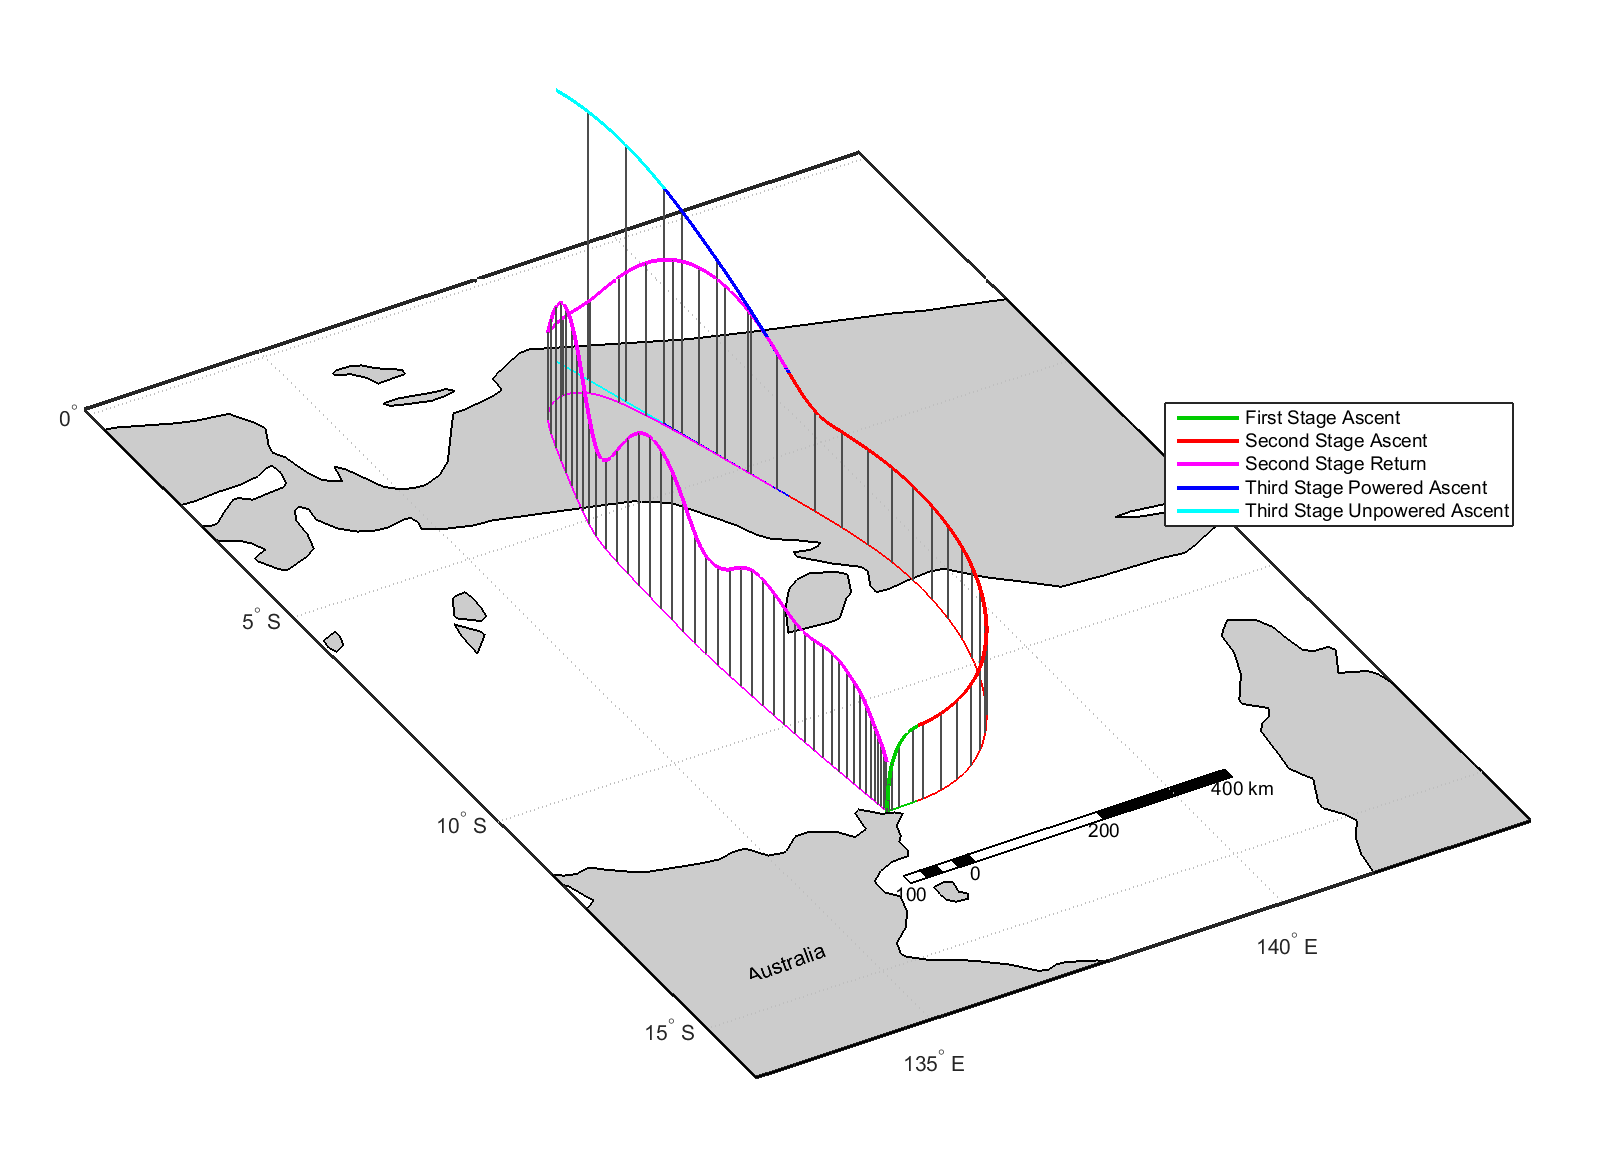
\includegraphics[width=1\linewidth]{../LODESTAR_FINAL/Results/mode10/GroundTrackStandard}
	\caption{The optimised maximum payload-to-orbit trajectory of the launch system (Case 2).}
	\label{fig:GroundTrackStandardNoReturn}
\end{figure}


The first stage trajectory, shown in Figure \ref{fig:FirstStageStandardNoReturn}, has a very similar trajectory shape to that of the first stage releasing the SPARTAN onto a constant dynamic pressure trajectory.
\begin{figure}[ht!]
	\centering
	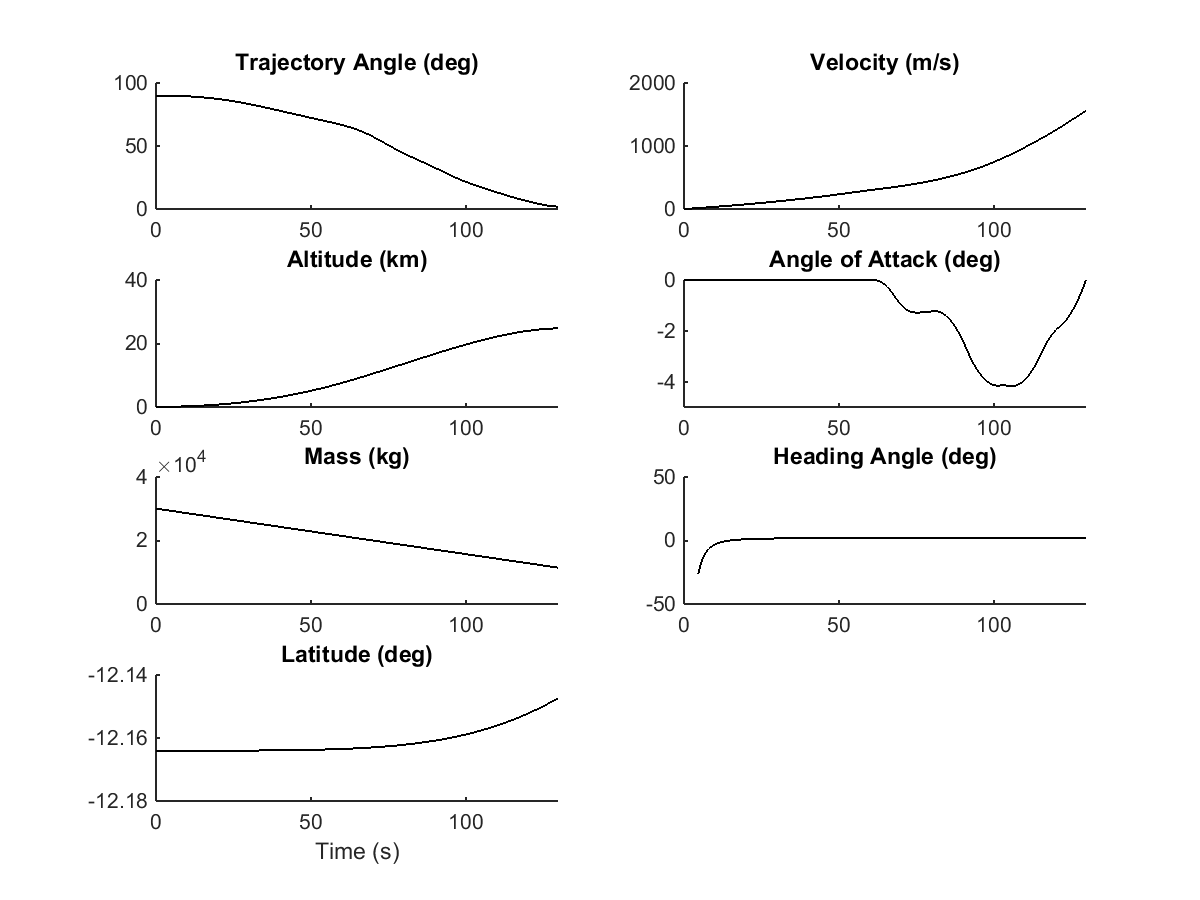
\includegraphics[width=0.9\linewidth]{../LODESTAR_FINAL/Results/mode10/FirstStageStandard}
	\caption{The optimised maximum payload-to-orbit trajectory of the launch system under power of the first stage rocket (Case 2).}
	\label{fig:FirstStageStandardNoReturn}
\end{figure}
 However, the trajectory angle at the separation of the SPARTAN is \secondthirdSeparationgammaqStandardNoReturn$^\circ$, rather than the trajectory angle of \secondthirdSeparationgammaConstq$^\circ$ required for the SPARTAN to fly a constant dynamic pressure trajectory. This higher release angle causes the altitude of the SPARTAN to immediately increase, and consequently for its dynamic pressure to decrease. This trajectory angle at release is the consequence of a trade-off between the efficiency of the SPARTAN and the first stage efficiency. The efficiency of the first stage is increased to 8.171\%, an overall improvement of 0.161\% compared to the first stage separating the SPARTAN at 50kPa conditions. 
 
 In addition to improving the exergy efficiency of the first stage, the higher release angle and altitude conditions also allow the first stage to launch with more fuel. In order to release the SPARTAN at a trajectory angle conducive to flying at 50kPa, the first stage must launch with a low fuel mass, to allow it to pitch in the correct manner. When the SPARTAN release angle and altitude are increased during the maximum payload-to-orbit trajectory, the first stage is able to launch with a fuel mass of 17185kg, an increase of 1.0\% compared to the constant dynamic pressure trajectory in Case 1. During the maximum payload-to-orbit trajectory, the first stage rocket releases the SPARTAN at a velocity of 1484.3m/s, an increase of 2.7\% compared to the first stage releasing the SPARTAN onto a constant dynamic pressure trajectory. Neither first stage utilises the full amount of allowable fuel mass, 17934kg, indicating that using the full fuel mass would necessitate separation conditions which would reduce the efficiency of the SPARTAN unfavourably. 
These results indicate that the fuel mass utilised by the first stage has a distinct optimal magnitude, and that including additional fuel over a certain amount may not increase the performance of the system. This implies that the size of the first stage is closely linked to the optimal trajectory of the system, and that future first stage designs should be sized so that optimal pitching is achieved. 

\begin{table}[ht]
	\centering
\begin{tabular}{l c } 
	\hline \textbf{Trajectory Condition}
	& StandardNoReturn

	\\
	\hline \textbf{Payload to Orbit (kg)}
	& \textbf{\PayloadToOrbitStandardNoReturn}
	\\
	\textbf{Total $\eta_{exergy}$ (\%)}
	& \textbf{\totalExergyEffStandardNoReturn}
	\\
	\hline 
	\textbf{1$^{st}$ Stage $\eta_{exergy}$ (\%)}
	& \textbf{\firstExergyEffStandardNoReturn}
	\\
	\textbf{Separation Alt, 1$\rightarrow$2 (km)}
	& \firstsecondSeparationAltStandardNoReturn
	\\
	\textbf{Separation v, 1$\rightarrow$2 (m/s)}
	& \firstsecondSeparationvStandardNoReturn
	\\
	\textbf{Separation $\gamma$, 1$\rightarrow$2 (m/s)}
	& \firstsecondSeparationgammaStandardNoReturn
	\\
	\hline 
	\textbf{2$^{nd}$ Stage $\eta_{exergy}$ (\%)}
	& \textbf{\secondExergyEffStandardNoReturn}
	\\
	\textbf{Separation Alt, 2$\rightarrow$3 (km)}
	& \secondthirdSeparationAltStandardNoReturn
	\\
	\textbf{Separation $v$, 2$\rightarrow$3 (m/s)}
	& \secondthirdSeparationvStandardNoReturn
	\\
	\textbf{Separation $\gamma$, 2$\rightarrow$3 (deg)}
	& \secondthirdSeparationgammaStandardNoReturn
	\\
	\textbf{Separation $q$, 2$\rightarrow$3(kPa)}
	& \secondthirdSeparationqStandardNoReturn
	\\
	\textbf{2$^{nd}$ Stage L/D, 2$\rightarrow$3}
	& \secondthirdSeparationLDStandardNoReturn
	\\
	\textbf{2$^{nd}$ Stage Flight Time (s)}
	& \secondFlightTimeStandardNoReturn
	\\
	\hline 
	\textbf{3$^{rd}$ Stage $\eta_{exergy}$ (\%)}
	& \textbf{\thirddExergyEffStandardNoReturn}
	\\
	\textbf{3$^{rd}$ Stage $t$, $q >$ 5kpa (s)}
	& \thirdqOverFiveStandardNoReturn
	\\
	\textbf{3$^{rd}$ Stage max $\alpha$ (deg)}
	& \thirdmaxAoAStandardNoReturn
	\\
	\textbf{3$^{rd}$ Stage Fuel Mass (kg)}
	& \thirdmFuelStandardNoReturn
	\\
	\hline 
\end{tabular} 
	\caption{A summary of key results from the maximum payload-to-orbit trajectory (Case 2).}
	\label{tab:summaryStandardNoReturn}
\end{table}







\begin{figure}[ht!]
\centering
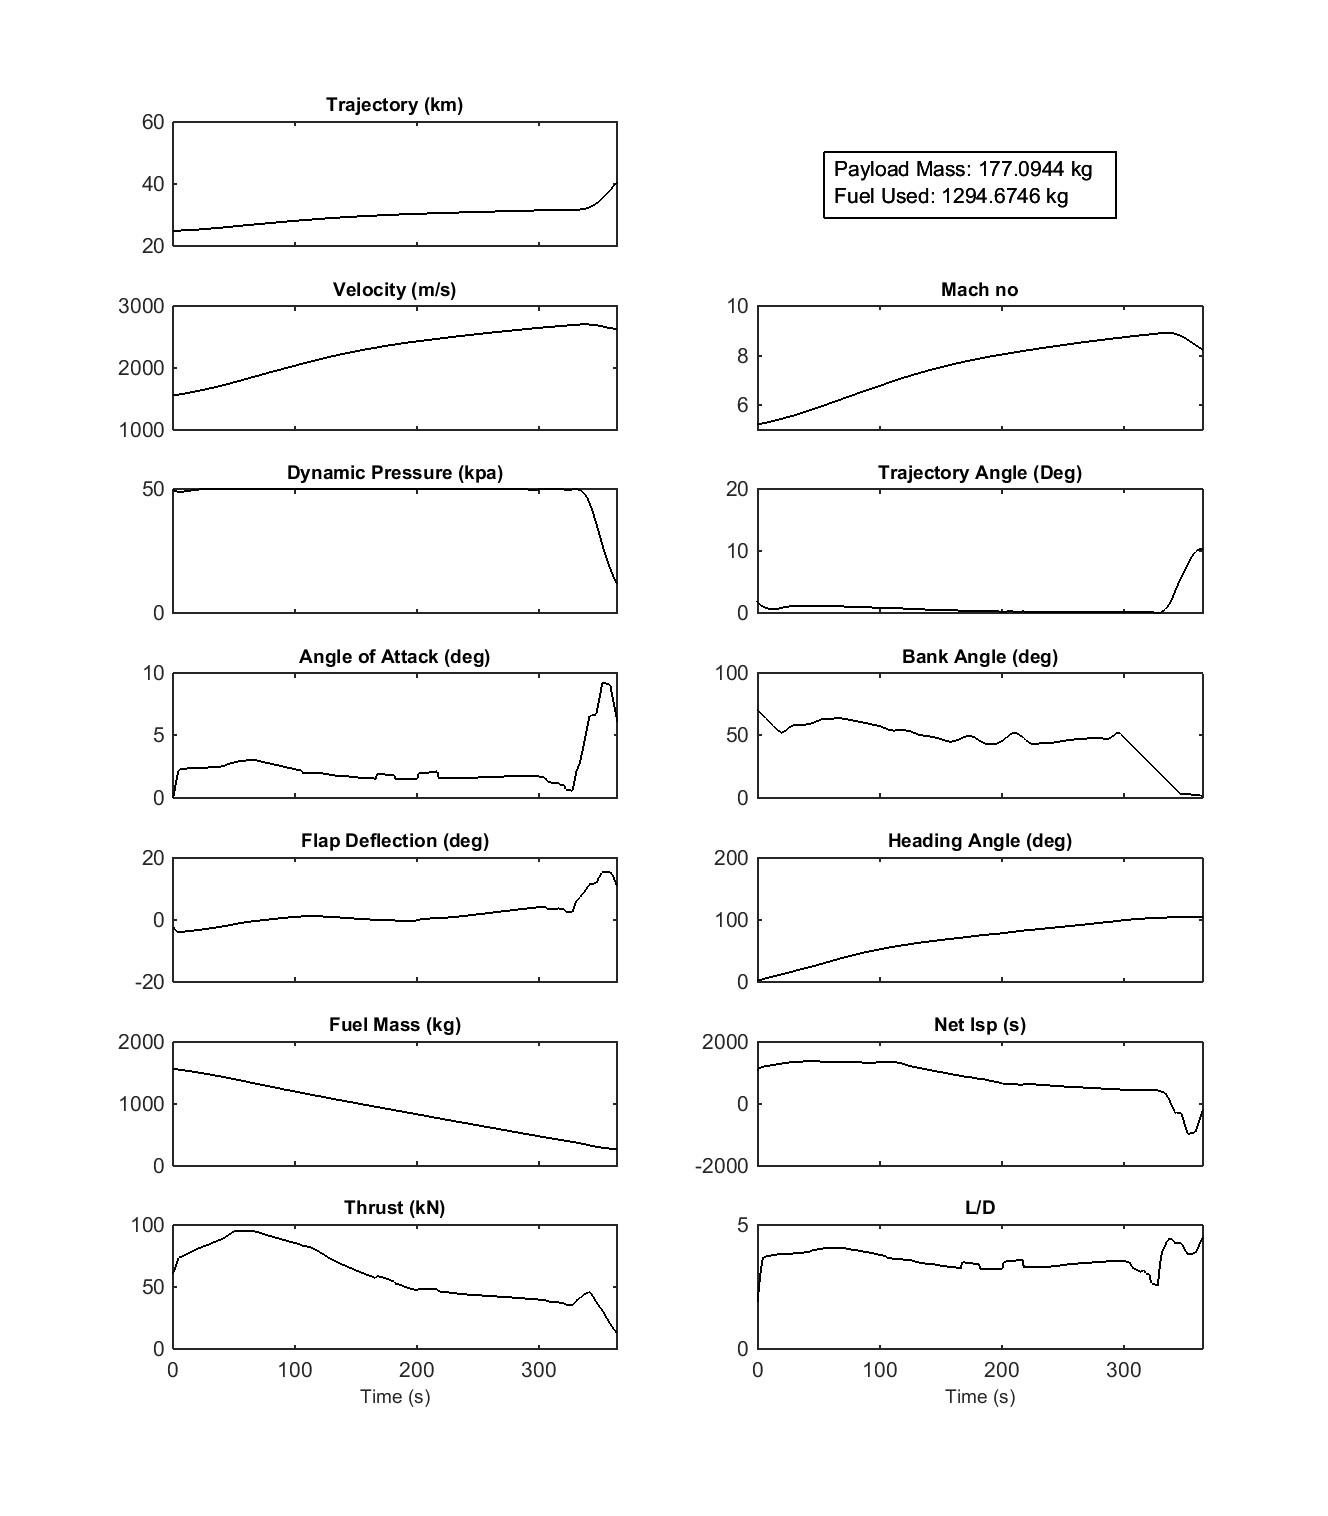
\includegraphics[width=0.9\linewidth]{../LODESTAR_FINAL/Results/mode10/SecondStageStandard}
\caption{The optimised maximum payload-to-orbit of the SPARTAN (Case 2).}
\label{fig:SecondStageStandardNoReturn}
\end{figure}



After the initial deviation from the maximum dynamic pressure, the SPARTAN returns to 50kPa dynamic pressure for a time. 
At 122.5 seconds, the altitude of the trajectory is again raised, and the dynamic pressure decreased, to a minimum of 35.6kPa. In this region the net specific impulse of the SPARTAN is relatively homogeneous with respect to changes in dynamic pressure. This homogeneous region can be observed in the specific impulse of the C-REST engines in Figure \ref{fig:IspStandard}, between inlet Mach number (M1) values of 6 and 7, and in Figure \ref{fig:NetIspStandardNoReturn}, in the Mach 7 and 8 plots of net specific impulse. This homogeneity means that the variation in engine performance with flight conditions is small and that flying at the maximum dynamic pressure in this region does not maximise the specific impulse from the C-REST engines. Figure \ref{fig:NetIspStandardNoReturn} shows that while the optimised trajectory differs significantly from a constant dynamic pressure trajectory, both achieve similar net specific impulses, with the exception of the initial trajectory conditions at Mach 5, where the efficiency of the SPARTAN is traded for first stage rocket performance. 


Appendix \ref{sec:Appendix_qconst} details a maximum payload-to-orbit trajectory in which the trajectory is constrained to 50kPa between Mach 6-8, to prevent the altitude raising manoeuvre from taking place, for comparison. 
The altitude raising manoeuvre
increases the combined total efficiency launch system from \totalExergyEffqconstrained \% to \totalExergyEffStandardNoReturn \% (calculated including stage separations). This is a relatively minor variation, and the payload-to-orbit benefits of this altitude raising manoeuvre are correspondingly small. 
The optimised trajectory exhibits a payload-to-orbit increase of 0.4kg compared to the trajectory constrained to 50kPa between Mach 6-8, a difference of only 0.2\%.
However, it is important to note that, while its benefits are small, the altitude raising manoeuvre is consistently observed in every maximum payload-to-orbit optimised trajectory. 
Also, though its benefits to payload-to-orbit are small, this altitude raising manoeuvre is significant as it reduces the heating and structural loading on the SPARTAN, though it is beyond the scope of this study to quantify these benefits. 




\begin{figure}[ht!]
	\centering
	\includegraphics[width=0.8\linewidth]{../LODESTAR_FINAL/Results/mode10/NetIspStandard}
	\caption{Net Isp contours for the SPARTAN at Mach numbers from 5-9, showing optimised trajectory and constant dynamic pressure trajectory.}
	\label{fig:NetIspStandardNoReturn}
\end{figure}

\begin{figure}[ht!]
	\centering
	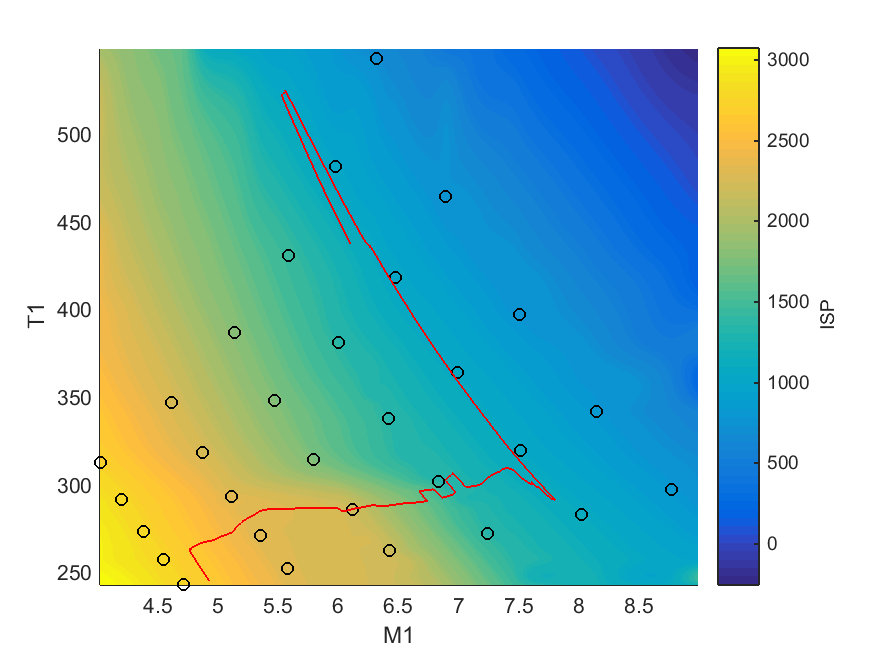
\includegraphics[width=0.8\linewidth]{../LODESTAR_FINAL/Results/mode10/IspStandard}
	\caption{The specific impulse of the C-REST engines, plotted for inlet temperature (T1) and inlet Mach number (M1). Data points are shown in black.}
	\label{fig:IspStandard}
\end{figure}


At 314.3s, the SPARTAN returns to flight at close to 50kPa dynamic pressure until 494.1s at which point a pull-up manoeuvre is performed, gaining altitude until the third stage rocket is released at 528.4s SPARTAN flight time. 
 The point at which the pull-up manoeuvre begins is the optimisation result that takes into account the best combination of velocity, altitude and release angle for scramjet stage performance and the release of the rocket stage. This pull-up indicates the region at which increasing altitude and release angle becomes more important than extracting maximum thrust from the scramjet (which is generally attained at high $q$ and low flight angle at an equivalence ratio of 1).
At high Mach numbers, flight in a lower dynamic pressure environment results in less thrust output from the scramjet engines, as well as an increase in angle of attack and flap deflection angle to compensate for the additional lift required. Due to this, less overall acceleration is obtained compared to the constant dynamic pressure result with minimum pull-up. Separation occurs at a velocity of \secondthirdSeparationvStandardNoReturn m/s, a decrease of 116.2m/s. However, at the same time separation altitude increases by 9.48km to \secondthirdSeparationAltqStandardNoReturn km, resulting in a decrease in separation dynamic pressure to \secondthirdSeparationqStandardNoReturn kPa. 
\begin{figure}[ht!]
	\centering
	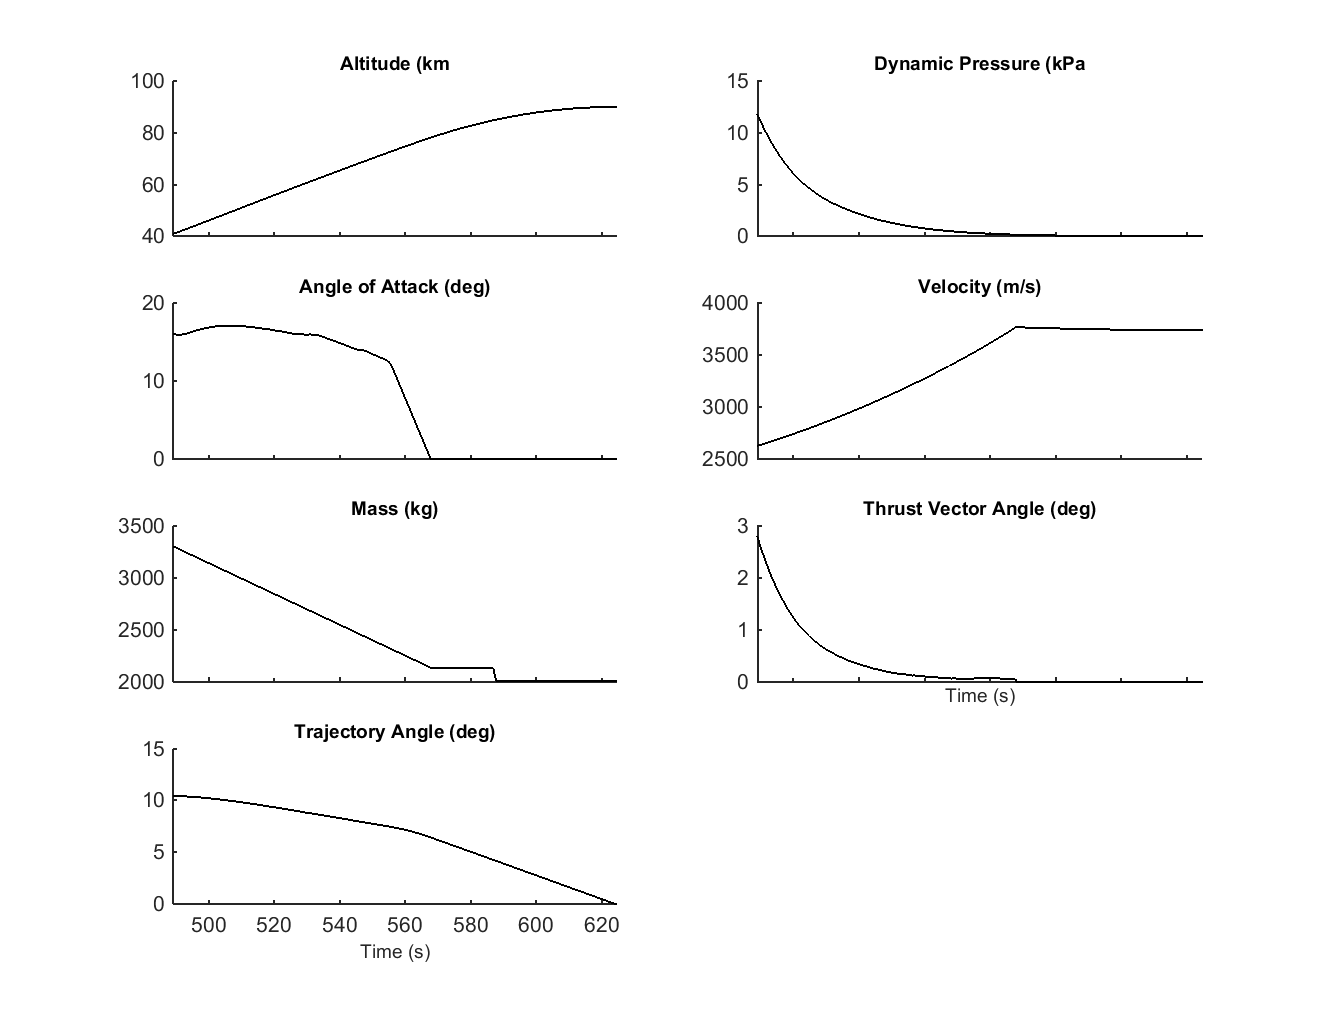
\includegraphics[width=0.9\linewidth]{../LODESTAR_FINAL/Results/mode10/ThirdStageStandard}
	\caption{The third stage trajectory of the launch system flying the maximum payload-to-orbit trajectory (Case 2).}
	\label{fig:ThirdStageStandardNoReturn}
\end{figure}
The larger scramjet stage pull-up assists the rocket in manoeuvring to exoatmospheric altitude by increasing the altitude and angle at separation by utilising the increased L/D ratio and manoeuvrability of the scramjet vehicle. The increase in release angle, to the optimal angle of \secondthirdSeparationgammaStandardNoReturn$^\circ$, significantly reduces the turning that is required by the rocket as evident from comparing Fig \ref{fig:ThirdStageConstq} and \ref{fig:ThirdStageStandardNoReturn}. 
Overall, the altitude raising manoeuvres which the SPARTAN performs result in a decrease in the exergy efficiency of the SPARTAN to \secondExergyEffStandardNoReturn \%, a total decrease of 1.318\% compared to the SPARTAN flying at a constant dynamic pressure. However, the optimised trajectory drastically increases the exergy efficiency of the third stage, to \thirddExergyEffStandardNoReturn \%, an overall increase of 6.72 \% compared to the third stage released from the SPARTAN flying a constant dynamic pressure trajectory, so that the third stage is utilising its available energy 1.61 times as efficiently.  
This leads to the total exergy efficiency of the launch system increasing from \totalExergyEffConstq \% to \totalExergyEffStandardNoReturn \%. 

The trajectory of the third stage rocket after release from an optimised scramjet trajectory is shown in Figure \ref{fig:ThirdStageStandardNoReturn}. Release at a higher, more optimal angle reduces the aerodynamic moment, in turn reducing the necessary thrust vector angle so that the thrust vector limit is not reached. The third stage rocket is released at a high trajectory angle, and continuously gains altitude, avoiding the close-to-horizontal flight required by the fixed dynamic pressure release (Case 1).
Due to the higher altitude and release angle, the third stage rocket is released at a lower dynamic pressure, \secondthirdSeparationqCdStandardNoReturn kPa compared to \secondthirdSeparationqConstq kPa, and spends much less time flying in a high dynamic pressure environment, \thirdqOverFiveStandard s at over 5kPa dynamic pressure rather than \thirdqOverFiveConstq s. 
The reduced time that the rocket must spend in a high dynamic pressure environment and decrease in the maximum dynamic pressure that the rocket stage experiences may allow the structural mass and heat shielding necessary to achieve exoatmospheric flight to be decreased. This may enable higher payload to orbit, though it is beyond the scope of this study to investigate these design changes. 


Compared to studies considering vehicles with a scramjet-rocket transition within a single stage\cite{Lu1993,Trefny1999}[CITEXX], the maximum payload to orbit trajectory of the multi-stage system shows a scramjet-rocket transition point at much lower altitudes.
This lower transition point is a consequence of the stage separation creating an energy trade-off, which does not occur in a single stage vehicle. Single-stage vehicles must necessarily transport all components to exoatmosphere, and so utilise the scramjet engines until higher altitude to take advantage of their high efficiency. A multi-stage vehicle is able to separate the scramjet stage. 
This separation occurs when the performance benefits provided by the superior aerodynamics and engine efficiency of the scramjet stage are offset by the energy required to lift the extra mass to higher altitude. The beneficial ability
to separate the scramjet stage results in a lower altitude scramjet-rocket transition point, when compared to single
stage vehicle designs.



\section{Sensitivity Analysis}\label{sec:sensitivityNoReturn}


A sensitivity analysis is conducted, in which selected design parameters of the launch system are varied, and the effects on the optimised maximum payload-to-orbit trajectory of the launch system are investigated. Appendix \ref{sec:Appendix_trajectorycomparisons} shows comparison plots of the second and third stage trajectories for each parameter variation study, however, the first stage rocket trajectories are very similar and are not shown graphically. Key results including performance factors of each stage and separation conditions are summarised within this section.
This study is performed in order to determine the relative importance of the design parameters on the efficiency of the system, as well as investigating how the maximum payload-to-orbit trajectory changes as the performance of the launch system is varied. The investigation of the key design parameters of the launch system provides a metric which is used to quantify the relative impact of the vehicle design on the performance of the launch system. The performance trade-offs between the stages are investigated by studying the variation in the optimised trajectory as the vehicle design parameters are changed. 
Trends are developed for each parameter study, quantifying how much the performance factors of the launch system vary per percentage of variation of each design parameter ($\Delta$/\%). This percentage variation gives a general metric for how much each design parameter effects the performance factors of the launch system, however, the relative magnitude of one percent variation of each individual design parameter must be taken into account when making comparisons. 
The information obtained from this parameter variation study can be used to inform future launch system designs. 

For some of the trajectory simulations within this section, it is assumed that the scramjet engines are operable at velocities slightly under Mach 5, in order to allow meaningful assessment of parameters which effect the first stage-SPARTAN separation velocity, without modification of the first stage rocket.
All optimised trajectories within this section use the full amount of fuel available to the SPARTAN vehicle. 



\subsection{Case 3: Dynamic Pressure Sensitivity}\label{sec:qvariation}

To investigate the sensitivity of the vehicle to changes in $q_{max}$, the maximum dynamic pressure is varied by $\pm$10kPa in 5kPa increments, and the flight trajectory optimised, with results shown in Table \ref{tab:qvarnoreturn}.
The variation in maximum dynamic pressure has only a small effect on the total exergy efficiency of the system, and hence only a small effect on the payload mass delivered to heliocentric orbit.  Varying the maximum dynamic pressure by $\pm20\%$ causes a variation of only +0.065\% or -0.069\% in exergy efficiency and a corresponding +7.2kg (+3.8\%) or -7.8kg (-4.1\%) variation in payload to orbit.  
Separation altitudes of \secondthirdSeparationAltqFortyNoReturn km and \secondthirdSeparationAltqSixtyNoReturn km are reached for the 40kPa and 60kPa limited cases respectively, with separation velocities of \secondthirdSeparationvqFortyNoReturn m/s and \secondthirdSeparationvqSixtyNoReturn m/s. The 40kPa limited case flies for \secondFlightTimeqFortyNoReturn s, significantly longer than the 60kPa case which flies for \secondFlightTimeqSixtyNoReturn s.
As the dynamic pressure decreases, the size of the altitude raising manoeuvre in the middle of the trajectory lessens. This is due to the increased altitude and angle of attack moving the flight conditions into a region where the specific impulse of the C-REST engines is not homogeneous, so that it is beneficial to fly at maximum dynamic pressure.  
All trajectories pull-up to similar altitudes, with relatively small variation in separation velocity.
This small variation in velocity is despite the increase in air density and decrease in angle of attack required for flight at higher dynamic pressures, both of which increase the mass flow into the engine. Although the thrust output of the REST engines increases with dynamic pressure, so does the drag on the vehicle, and the net increase in performance is relatively small (0.02 $\Delta\eta_{exergy}$/$\Delta$\%q). 
The trade-off between the exergy efficiency of the first and second stages shifts as the dynamic pressure limit is increased, with the first stage rocket becoming less efficient (varying from an $\eta_{exergy}$ of \firstExergyEffqFortyNoReturn \% at 40kPa to \firstExergyEffqSixtyNoReturn \% at 60kPa), while the exergy efficiency of the SPARTAN increases (varying from an $\eta_{exergy}$ of \secondExergyEffqFortyNoReturn \% at 40kPa to \secondExergyEffqSixtyNoReturn \% at 60kPa). The decreased altitude of first stage-SPARTAN separation requires the first stage to pitch more to reach the optimal staging conditions, resulting in a less efficient first stage trajectory, which partially offsets some of the increased SPARTAN performance gained from the flight at higher dynamic pressure. 

\begin{table}[ht]
	\centering
\begin{tabular}{l c c c c c c} 
	\hline \textbf{Trajectory Condition}
	&q40
	&q45
	&q
	&q55
	&q60
	& $\Delta/\Delta$\%q
	\\
	\hline \textbf{Payload to Orbit (kg)}
	& \textbf{\PayloadToOrbitqFortyNoReturn}
	& \textbf{\PayloadToOrbitqFortyFiveNoReturn}
	& \textbf{\PayloadToOrbitqStandardNoReturn}
	& \textbf{\PayloadToOrbitqFiftyFiveNoReturn}
	& \textbf{\PayloadToOrbitqSixtyNoReturn}
	&\textbf{0.4}
	\\
	\textbf{Payload Variation (\%)}
	& \PayloadVarqFortyNoReturn
	& \PayloadVarqFortyFiveNoReturn
	& \PayloadVarqStandardNoReturn
	& \PayloadVarqFiftyFiveNoReturn
	& \PayloadVarqSixtyNoReturn
	&0.2
	\\
	\textbf{Total $\eta_{exergy}$ (\%)}
	& \textbf{\totalExergyEffqFortyNoReturn}
	& \textbf{\totalExergyEffqFortyFiveNoReturn}
	& \textbf{\totalExergyEffqStandardNoReturn}
	& \textbf{\totalExergyEffqFiftyFiveNoReturn}
	& \textbf{\totalExergyEffqSixtyNoReturn}
	& \textbf{3e-05}
	\\
	\hline 
	\textbf{1$^{st}$ Stage $\eta_{exergy}$ (\%)}
	& \textbf{\firstExergyEffqFortyNoReturn}
	& \textbf{\firstExergyEffqFortyFiveNoReturn}
	& \textbf{\firstExergyEffqStandardNoReturn}
	& \textbf{\firstExergyEffqFiftyFiveNoReturn}
	& \textbf{\firstExergyEffqSixtyNoReturn}
	& \textbf{-0.003}
	\\
	\textbf{Separation Alt, 1$\rightarrow$2 (km)}
	& \firstsecondSeparationAltqFortyNoReturn
	& \firstsecondSeparationAltqFortyFiveNoReturn
	& \firstsecondSeparationAltqStandardNoReturn
	& \firstsecondSeparationAltqFiftyFiveNoReturn
	& \firstsecondSeparationAltqSixtyNoReturn
	&-0.06
	\\
	\textbf{Separation v, 1$\rightarrow$2 (m/s)}
	& \firstsecondSeparationvqFortyNoReturn
	& \firstsecondSeparationvqFortyFiveNoReturn
	& \firstsecondSeparationvqStandardNoReturn
	& \firstsecondSeparationvqFiftyFiveNoReturn
	& \firstsecondSeparationvqSixtyNoReturn
	& -
	\\
	\textbf{Separation $\gamma$, 1$\rightarrow$2 (m/s)}
	& \firstsecondSeparationgammaqFortyNoReturn
	& \firstsecondSeparationgammaqFortyFiveNoReturn
	& \firstsecondSeparationgammaqStandardNoReturn
	& \firstsecondSeparationgammaqFiftyFiveNoReturn
	& \firstsecondSeparationgammaqSixtyNoReturn
	&-0.13
	\\
	\hline 
	\textbf{2$^{nd}$ Stage $\eta_{exergy}$ (\%)}
	& \textbf{\secondExergyEffqFortyNoReturn}
	& \textbf{\secondExergyEffqFortyFiveNoReturn}
	& \textbf{\secondExergyEffqStandardNoReturn}
	& \textbf{\secondExergyEffqFiftyFiveNoReturn}
	& \textbf{\secondExergyEffqSixtyNoReturn}
	& \textbf{0.02}
	\\
	\textbf{Separation Alt, 2$\rightarrow$3 (km)}
	& \secondthirdSeparationAltqFortyNoReturn
	& \secondthirdSeparationAltqFortyFiveNoReturn
	& \secondthirdSeparationAltqStandardNoReturn
	& \secondthirdSeparationAltqFiftyFiveNoReturn
	& \secondthirdSeparationAltqSixtyNoReturn
	&-0.02
	\\
	\textbf{Separation $v$, 2$\rightarrow$3 (m/s)}
	& \secondthirdSeparationvqFortyNoReturn
	& \secondthirdSeparationvqFortyFiveNoReturn
	& \secondthirdSeparationvqStandardNoReturn
	& \secondthirdSeparationvqFiftyFiveNoReturn
	& \secondthirdSeparationvqSixtyNoReturn
	&1.56
	\\
	\textbf{Separation $\gamma$, 2$\rightarrow$3 (deg)}
	& \secondthirdSeparationgammaqFortyNoReturn
	& \secondthirdSeparationgammaqFortyFiveNoReturn
	& \secondthirdSeparationgammaqStandardNoReturn
	& \secondthirdSeparationgammaqFiftyFiveNoReturn
	& \secondthirdSeparationgammaqSixtyNoReturn
	&0.03
	\\
	\textbf{Separation $q$, 2$\rightarrow$3(kPa)}
	& \secondthirdSeparationqqFortyNoReturn
	& \secondthirdSeparationqqFortyFiveNoReturn
	& \secondthirdSeparationqqStandardNoReturn
	& \secondthirdSeparationqqFiftyFiveNoReturn
	& \secondthirdSeparationqqSixtyNoReturn
	&0.04
	\\
	\textbf{2$^{nd}$ Stage L/D, 2$\rightarrow$3}
	& \secondthirdSeparationLDqFortyNoReturn
	& \secondthirdSeparationLDqFortyFiveNoReturn
	& \secondthirdSeparationLDqStandardNoReturn
	& \secondthirdSeparationLDqFiftyFiveNoReturn
	& \secondthirdSeparationLDqSixtyNoReturn
	& -
	\\
	\textbf{2$^{nd}$ Stage Flight Time (s)}
	& \secondFlightTimeqFortyNoReturn
	& \secondFlightTimeqFortyFiveNoReturn
	& \secondFlightTimeqStandardNoReturn
	& \secondFlightTimeqFiftyFiveNoReturn
	& \secondFlightTimeqSixtyNoReturn
	&-3.62
	\\
	\hline 
	\textbf{3$^{rd}$ Stage $\eta_{exergy}$ (\%)}
	& \textbf{\thirddExergyEffqFortyNoReturn}
	& \textbf{\thirddExergyEffqFortyFiveNoReturn}
	& \textbf{\thirddExergyEffqStandardNoReturn}
	& \textbf{\thirddExergyEffqFiftyFiveNoReturn}
	& \textbf{\thirddExergyEffqSixtyNoReturn}
	& -
	\\
	\textbf{3$^{rd}$ Stage $t$, $q >$ 5kpa (s)}
	& \thirdqOverFiveqFortyNoReturn
	& \thirdqOverFiveqFortyFiveNoReturn
	& \thirdqOverFiveqStandardNoReturn
	& \thirdqOverFiveqFiftyFiveNoReturn
	& \thirdqOverFiveqSixtyNoReturn
	& -
	\\
	\textbf{3$^{rd}$ Stage max $\alpha$ (deg)}
	& \thirdmaxAoAqFortyNoReturn
	& \thirdmaxAoAqFortyFiveNoReturn
	& \thirdmaxAoAqStandardNoReturn
	& \thirdmaxAoAqFiftyFiveNoReturn
	& \thirdmaxAoAqSixtyNoReturn
	&0
	\\
	\textbf{3$^{rd}$ Stage Fuel Mass (kg)}
	& \thirdmFuelqFortyNoReturn
	& \thirdmFuelqFortyFiveNoReturn
	& \thirdmFuelqStandardNoReturn
	& \thirdmFuelqFiftyFiveNoReturn
	& \thirdmFuelqSixtyNoReturn
	&-0.37
	\\
	\hline 
\end{tabular} 
 \caption{}
 \label{tab:qvarnoreturn}
\end{table}





\subsection{Case 4: SPARTAN Drag Sensitivity}\label{sec:dragvariation}

\begin{table}[ht!]
	\centering
	\begin{tabular}{l c c c c c c} 
		\hline \textbf{Trajectory Condition}
		&Cd90
		&Cd95
		&Cd
		&Cd105
		&Cd110
		& /\%
		\\
		\hline \textbf{Payload to Orbit (kg)}
		& \textbf{\PayloadToOrbitCdNinetyNoReturn}
		& \textbf{\PayloadToOrbitCdNinetyFiveNoReturn}
		& \textbf{\PayloadToOrbitCdStandardNoReturn}
		& \textbf{\PayloadToOrbitCdOneHundredFiveNoReturn}
		& \textbf{\PayloadToOrbitCdOneHundredTenNoReturn}
		&\textbf{-1.9}
		\\
		\textbf{Payload Variation (\%)}
		& \PayloadVarCdNinetyNoReturn
		& \PayloadVarCdNinetyFiveNoReturn
		& \PayloadVarCdStandardNoReturn
		& \PayloadVarCdOneHundredFiveNoReturn
		& \PayloadVarCdOneHundredTenNoReturn
		&-0.99
		\\
		\textbf{Total $\eta_{exergy}$ (\%)}
		& \textbf{\totalExergyEffCdNinetyNoReturn}
		& \textbf{\totalExergyEffCdNinetyFiveNoReturn}
		& \textbf{\totalExergyEffCdStandardNoReturn}
		& \textbf{\totalExergyEffCdOneHundredFiveNoReturn}
		& \textbf{\totalExergyEffCdOneHundredTenNoReturn}
		& \textbf{-0.00016}
		\\
		\hline 
		\textbf{1$^{st}$ Stage $\eta_{exergy}$ (\%)}
		& \textbf{\firstExergyEffCdNinetyNoReturn}
		& \textbf{\firstExergyEffCdNinetyFiveNoReturn}
		& \textbf{\firstExergyEffCdStandardNoReturn}
		& \textbf{\firstExergyEffCdOneHundredFiveNoReturn}
		& \textbf{\firstExergyEffCdOneHundredTenNoReturn}
		& \textbf{-0.041}
		\\
		\textbf{Separation Alt, 1$\rightarrow$2 (km)}
		& \firstsecondSeparationAltCdNinetyNoReturn
		& \firstsecondSeparationAltCdNinetyFiveNoReturn
		& \firstsecondSeparationAltCdStandardNoReturn
		& \firstsecondSeparationAltCdOneHundredFiveNoReturn
		& \firstsecondSeparationAltCdOneHundredTenNoReturn
		&-0.09
		\\
		\textbf{Separation v, 1$\rightarrow$2 (m/s)}
		& \firstsecondSeparationvCdNinetyNoReturn
		& \firstsecondSeparationvCdNinetyFiveNoReturn
		& \firstsecondSeparationvCdStandardNoReturn
		& \firstsecondSeparationvCdOneHundredFiveNoReturn
		& \firstsecondSeparationvCdOneHundredTenNoReturn
		&-4.87
		\\
		\textbf{Separation $\gamma$, 1$\rightarrow$2 (m/s)}
		& \firstsecondSeparationgammaCdNinetyNoReturn
		& \firstsecondSeparationgammaCdNinetyFiveNoReturn
		& \firstsecondSeparationgammaCdStandardNoReturn
		& \firstsecondSeparationgammaCdOneHundredFiveNoReturn
		& \firstsecondSeparationgammaCdOneHundredTenNoReturn
		&-0.22
		\\
		\hline 
		\textbf{2$^{nd}$ Stage $\eta_{exergy}$ (\%)}
		& \textbf{\secondExergyEffCdNinetyNoReturn}
		& \textbf{\secondExergyEffCdNinetyFiveNoReturn}
		& \textbf{\secondExergyEffCdStandardNoReturn}
		& \textbf{\secondExergyEffCdOneHundredFiveNoReturn}
		& \textbf{\secondExergyEffCdOneHundredTenNoReturn}
		& \textbf{-0.086}
		\\
		\textbf{Separation Alt, 2$\rightarrow$3 (km)}
		& \secondthirdSeparationAltCdNinetyNoReturn
		& \secondthirdSeparationAltCdNinetyFiveNoReturn
		& \secondthirdSeparationAltCdStandardNoReturn
		& \secondthirdSeparationAltCdOneHundredFiveNoReturn
		& \secondthirdSeparationAltCdOneHundredTenNoReturn
		& -
		\\
		\textbf{Separation $v$, 2$\rightarrow$3 (m/s)}
		& \secondthirdSeparationvCdNinetyNoReturn
		& \secondthirdSeparationvCdNinetyFiveNoReturn
		& \secondthirdSeparationvCdStandardNoReturn
		& \secondthirdSeparationvCdOneHundredFiveNoReturn
		& \secondthirdSeparationvCdOneHundredTenNoReturn
		&-10.69
		\\
		\textbf{Separation $\gamma$, 2$\rightarrow$3 (deg)}
		& \secondthirdSeparationgammaCdNinetyNoReturn
		& \secondthirdSeparationgammaCdNinetyFiveNoReturn
		& \secondthirdSeparationgammaCdStandardNoReturn
		& \secondthirdSeparationgammaCdOneHundredFiveNoReturn
		& \secondthirdSeparationgammaCdOneHundredTenNoReturn
		& -
		\\
		\textbf{Separation $q$, 2$\rightarrow$3(kPa)}
		& \secondthirdSeparationqCdNinetyNoReturn
		& \secondthirdSeparationqCdNinetyFiveNoReturn
		& \secondthirdSeparationqCdStandardNoReturn
		& \secondthirdSeparationqCdOneHundredFiveNoReturn
		& \secondthirdSeparationqCdOneHundredTenNoReturn
		& -
		\\
		\textbf{2$^{nd}$ Stage L/D, 2$\rightarrow$3}
		& \secondthirdSeparationLDCdNinetyNoReturn
		& \secondthirdSeparationLDCdNinetyFiveNoReturn
		& \secondthirdSeparationLDCdStandardNoReturn
		& \secondthirdSeparationLDCdOneHundredFiveNoReturn
		& \secondthirdSeparationLDCdOneHundredTenNoReturn
		&-0.02
		\\
		\textbf{2$^{nd}$ Stage Flight Time (s)}
		& \secondFlightTimeCdNinetyNoReturn
		& \secondFlightTimeCdNinetyFiveNoReturn
		& \secondFlightTimeCdStandardNoReturn
		& \secondFlightTimeCdOneHundredFiveNoReturn
		& \secondFlightTimeCdOneHundredTenNoReturn
		& -
		\\
		\hline 
		\textbf{3$^{rd}$ Stage $\eta_{exergy}$ (\%)}
		& \textbf{\thirddExergyEffCdNinetyNoReturn}
		& \textbf{\thirddExergyEffCdNinetyFiveNoReturn}
		& \textbf{\thirddExergyEffCdStandardNoReturn}
		& \textbf{\thirddExergyEffCdOneHundredFiveNoReturn}
		& \textbf{\thirddExergyEffCdOneHundredTenNoReturn}
		& \textbf{0.047}
		\\
		\textbf{3$^{rd}$ Stage $t$, $q >$ 5kpa (s)}
		& \thirdqOverFiveCdNinetyNoReturn
		& \thirdqOverFiveCdNinetyFiveNoReturn
		& \thirdqOverFiveCdStandardNoReturn
		& \thirdqOverFiveCdOneHundredFiveNoReturn
		& \thirdqOverFiveCdOneHundredTenNoReturn
		& -
		\\
		\textbf{3$^{rd}$ Stage max $\alpha$ (deg)}
		& \thirdmaxAoACdNinetyNoReturn
		& \thirdmaxAoACdNinetyFiveNoReturn
		& \thirdmaxAoACdStandardNoReturn
		& \thirdmaxAoACdOneHundredFiveNoReturn
		& \thirdmaxAoACdOneHundredTenNoReturn
		& -
		\\
		\textbf{3$^{rd}$ Stage Fuel Mass (kg)}
		& \thirdmFuelCdNinetyNoReturn
		& \thirdmFuelCdNinetyFiveNoReturn
		& \thirdmFuelCdStandardNoReturn
		& \thirdmFuelCdOneHundredFiveNoReturn
		& \thirdmFuelCdOneHundredTenNoReturn
		&1.86
		\\
		\hline 
	\end{tabular} 
	\caption{}
	\label{tab:DragVariationNoReturn}
\end{table}

To investigate the effect of the vehicle design and uncertainty in aerodynamic performance on the optimal trajectory the drag of the SPARTAN is varied by $\pm10$\%, and an optimised trajectory calculated with dynamic pressure limited to 50kpa. Results are compared to the 100\% drag result in \ref{tab:DragVariationNoReturn} with a trajectory path comparison shown in Appendix \ref{sec:Appendix_trajectorycomparisons}. The drag of the SPARTAN is varied during both the first stage ascent, as well as the acceleration of the SPARTAN. 

The drag variation of the SPARTAN shows a significant effect on the overall efficiency of the system (+0.182\% at 90\% drag, and -0.147\% at 110\% drag) and correspondingly, on the maximum payload-to-orbit (+19.6kg at 90\% drag, a variation of +10.4\% and -17.2kg at 110\% drag, a variation of -9.1\%). The exergy efficiencies of the first stage rocket and the SPARTAN are decreased significantly as the drag is increased, from \firstExergyEffCdNinetyNoReturn\% and \secondExergyEffCdNinetyNoReturn\% respectively at 90\% drag, to \firstExergyEffCdOneHundredTenNoReturn\% and \secondExergyEffCdOneHundredTenNoReturn\% respectively at 110\% drag. This reduction in efficiency is due to the energy which must be used to overcome the added drag. 
The velocity and trajectory angle at first stage-SPARTAN separation decrease significantly as the drag is increased. This indicates that the first stage is able to pitch more during the trajectory, as a consequence of accelerating more slowly as the drag increases.
The SPARTAN trajectory results show that when drag is varied, the optimal trajectories are similar to the base-line case, with a similarly sized pull-up, though as the drag is increased (ie. L/D is decreased), the second stage follows a slightly slower and hence lower flight path, and the SPARTAN generally pulls-up to a higher trajectory angle. The similar flight path shape of the high drag case suggests that sacrificing velocity to increase separation altitude in a pull-up manoeuvre is optimal for multiple vehicle designs, and that the size of this pull-up is consistent with variation in the aerodynamics of the SPARTAN.
As the drag of the SPARTAN increases, the exergy efficiency of the third stage shows a corresponding increase, from \thirddExergyEffCdNinetyNoReturn\% at 90\% drag, to \thirddExergyEffCdOneHundredTenNoReturn\% at 110\% drag. This indicates that as the performance of the SPARTAN is decreased, it is beneficial to trade-off more of the SPARTAN's performance for an increase in third stage efficiency, resulting in similarly sized pull-ups. 


\subsection{Case 5: C-REST Engine Specific Impulse Sensitivity}\label{sec:ispsensitivitynoflyback}

\begin{table}[ht!]
	\centering
	\begin{tabular}{l c c c c c c} 
		\hline \textbf{Trajectory Condition}
		&Isp90
		&Isp95
		&Isp
		&Isp105
		&Isp110
		& /\%
		\\
		\hline \textbf{Payload to Orbit (kg)}
		& \textbf{\PayloadToOrbitIspNinetyNoReturn}
		& \textbf{\PayloadToOrbitIspNinetyFiveNoReturn}
		& \textbf{\PayloadToOrbitIspStandardNoReturn}
		& \textbf{\PayloadToOrbitIspOneHundredFiveNoReturn}
		& \textbf{\PayloadToOrbitIspOneHundredTenNoReturn}
		&\textbf{2.2}
		\\
		\textbf{Payload Variation (\%)}
		& \PayloadVarIspNinetyNoReturn
		& \PayloadVarIspNinetyFiveNoReturn
		& \PayloadVarIspStandardNoReturn
		& \PayloadVarIspOneHundredFiveNoReturn
		& \PayloadVarIspOneHundredTenNoReturn
		&1.16
		\\
		\textbf{Total $\eta_{exergy}$ (\%)}
		& \textbf{\totalExergyEffIspNinetyNoReturn}
		& \textbf{\totalExergyEffIspNinetyFiveNoReturn}
		& \textbf{\totalExergyEffIspStandardNoReturn}
		& \textbf{\totalExergyEffIspOneHundredFiveNoReturn}
		& \textbf{\totalExergyEffIspOneHundredTenNoReturn}
		& \textbf{0.0002}
		\\
		\hline 
		\textbf{1$^{st}$ Stage $\eta_{exergy}$ (\%)}
		& \textbf{\firstExergyEffIspNinetyNoReturn}
		& \textbf{\firstExergyEffIspNinetyFiveNoReturn}
		& \textbf{\firstExergyEffIspStandardNoReturn}
		& \textbf{\firstExergyEffIspOneHundredFiveNoReturn}
		& \textbf{\firstExergyEffIspOneHundredTenNoReturn}
		& -
		\\
		\textbf{Separation Alt, 1$\rightarrow$2 (km)}
		& \firstsecondSeparationAltIspNinetyNoReturn
		& \firstsecondSeparationAltIspNinetyFiveNoReturn
		& \firstsecondSeparationAltIspStandardNoReturn
		& \firstsecondSeparationAltIspOneHundredFiveNoReturn
		& \firstsecondSeparationAltIspOneHundredTenNoReturn
		& -
		\\
		\textbf{Separation v, 1$\rightarrow$2 (m/s)}
		& \firstsecondSeparationvIspNinetyNoReturn
		& \firstsecondSeparationvIspNinetyFiveNoReturn
		& \firstsecondSeparationvIspStandardNoReturn
		& \firstsecondSeparationvIspOneHundredFiveNoReturn
		& \firstsecondSeparationvIspOneHundredTenNoReturn
		& -
		\\
		\textbf{Separation $\gamma$, 1$\rightarrow$2 (m/s)}
		& \firstsecondSeparationgammaIspNinetyNoReturn
		& \firstsecondSeparationgammaIspNinetyFiveNoReturn
		& \firstsecondSeparationgammaIspStandardNoReturn
		& \firstsecondSeparationgammaIspOneHundredFiveNoReturn
		& \firstsecondSeparationgammaIspOneHundredTenNoReturn
		& -
		\\
		\hline 
		\textbf{2$^{nd}$ Stage $\eta_{exergy}$ (\%)}
		& \textbf{\secondExergyEffIspNinetyNoReturn}
		& \textbf{\secondExergyEffIspNinetyFiveNoReturn}
		& \textbf{\secondExergyEffIspStandardNoReturn}
		& \textbf{\secondExergyEffIspOneHundredFiveNoReturn}
		& \textbf{\secondExergyEffIspOneHundredTenNoReturn}
		& \textbf{0.162}
		\\
		\textbf{Separation Alt, 2$\rightarrow$3 (km)}
		& \secondthirdSeparationAltIspNinetyNoReturn
		& \secondthirdSeparationAltIspNinetyFiveNoReturn
		& \secondthirdSeparationAltIspStandardNoReturn
		& \secondthirdSeparationAltIspOneHundredFiveNoReturn
		& \secondthirdSeparationAltIspOneHundredTenNoReturn
		& -
		\\
		\textbf{Separation $v$, 2$\rightarrow$3 (m/s)}
		& \secondthirdSeparationvIspNinetyNoReturn
		& \secondthirdSeparationvIspNinetyFiveNoReturn
		& \secondthirdSeparationvIspStandardNoReturn
		& \secondthirdSeparationvIspOneHundredFiveNoReturn
		& \secondthirdSeparationvIspOneHundredTenNoReturn
		&13.74
		\\
		\textbf{Separation $\gamma$, 2$\rightarrow$3 (deg)}
		& \secondthirdSeparationgammaIspNinetyNoReturn
		& \secondthirdSeparationgammaIspNinetyFiveNoReturn
		& \secondthirdSeparationgammaIspStandardNoReturn
		& \secondthirdSeparationgammaIspOneHundredFiveNoReturn
		& \secondthirdSeparationgammaIspOneHundredTenNoReturn
		&-0.08
		\\
		\textbf{Separation $q$, 2$\rightarrow$3(kPa)}
		& \secondthirdSeparationqIspNinetyNoReturn
		& \secondthirdSeparationqIspNinetyFiveNoReturn
		& \secondthirdSeparationqIspStandardNoReturn
		& \secondthirdSeparationqIspOneHundredFiveNoReturn
		& \secondthirdSeparationqIspOneHundredTenNoReturn
		& -
		\\
		\textbf{2$^{nd}$ Stage L/D, 2$\rightarrow$3}
		& \secondthirdSeparationLDIspNinetyNoReturn
		& \secondthirdSeparationLDIspNinetyFiveNoReturn
		& \secondthirdSeparationLDIspStandardNoReturn
		& \secondthirdSeparationLDIspOneHundredFiveNoReturn
		& \secondthirdSeparationLDIspOneHundredTenNoReturn
		& -
		\\
		\textbf{2$^{nd}$ Stage Flight Time (s)}
		& \secondFlightTimeIspNinetyNoReturn
		& \secondFlightTimeIspNinetyFiveNoReturn
		& \secondFlightTimeIspStandardNoReturn
		& \secondFlightTimeIspOneHundredFiveNoReturn
		& \secondFlightTimeIspOneHundredTenNoReturn
		& -
		\\
		\hline 
		\textbf{3$^{rd}$ Stage $\eta_{exergy}$ (\%)}
		& \textbf{\thirddExergyEffIspNinetyNoReturn}
		& \textbf{\thirddExergyEffIspNinetyFiveNoReturn}
		& \textbf{\thirddExergyEffIspStandardNoReturn}
		& \textbf{\thirddExergyEffIspOneHundredFiveNoReturn}
		& \textbf{\thirddExergyEffIspOneHundredTenNoReturn}
		& \textbf{-0.073}
		\\
		\textbf{3$^{rd}$ Stage $t$, $q >$ 5kpa (s)}
		& \thirdqOverFiveIspNinetyNoReturn
		& \thirdqOverFiveIspNinetyFiveNoReturn
		& \thirdqOverFiveIspStandardNoReturn
		& \thirdqOverFiveIspOneHundredFiveNoReturn
		& \thirdqOverFiveIspOneHundredTenNoReturn
		& -
		\\
		\textbf{3$^{rd}$ Stage max $\alpha$ (deg)}
		& \thirdmaxAoAIspNinetyNoReturn
		& \thirdmaxAoAIspNinetyFiveNoReturn
		& \thirdmaxAoAIspStandardNoReturn
		& \thirdmaxAoAIspOneHundredFiveNoReturn
		& \thirdmaxAoAIspOneHundredTenNoReturn
		& -
		\\
		\textbf{3$^{rd}$ Stage Fuel Mass (kg)}
		& \thirdmFuelIspNinetyNoReturn
		& \thirdmFuelIspNinetyFiveNoReturn
		& \thirdmFuelIspStandardNoReturn
		& \thirdmFuelIspOneHundredFiveNoReturn
		& \thirdmFuelIspOneHundredTenNoReturn
		&-2.2
		\\
		\hline 
	\end{tabular} 
	
\end{table}

The specific impulse of the C-REST scramjet engines is varied by $\pm10\%$ to directly investigate the effects of the efficiency of the scramjet engines on the performance of the launch vehicle. The maximum payload-to-orbit varies by +24.2kg (12.8\%) to -20.5kg (-10.8\%), and the total exergy efficiency varies by +0.220\% to -0.183\% at 110\% $I_{SP}$ and 90\% $I_{SP}$ respectively. 
The increased C-REST specific impulse does not vary the first stage performance significantly, and the first stage-SPARTAN separation point stays relatively constant for all cases excepting 110\% $I_{SP}$, where the altitude and trajectory angle of the first stage-SPARTAN separation increase. It is likely that this variation in release point at 110\% $I_{SP}$ is simply due to the optimiser converging to an optimal trajectory with slightly different trade-offs between the first stage and SPARTAN efficiency, but with similar overall efficiency.  
The small variations in first stage release point indicate that the efficiency trade-off between the first stage and the SPARTAN is not significantly affected by the efficiency of the SPARTAN, and is primarily driven by the capabilities of the first stage rocket. 
This is supported by the variability in the first stage-SPARTAN separation point when the mass or drag of the SPARTAN is changed, parameters which affect the ability of the first stage to pitch. 

The additional efficiency provided by increases the exergy efficiency of the SPARTAN considerably, by +1.724\% at 110\%$I_{SP}$ to -1.558\% at 90\% $I_{SP}$. 
Increasing the specific impulse of the C-REST engines allows the SPARTAN to accelerate more over the flight time, increasing the velocity at SPARTAN-third stage separation significantly. The velocity added to the end of the SPARTAN's trajectory directly contributes to the final velocity of the third stage at circularisation. Varying the specific impulse does not change the optimal SPARTAN-third stage separation altitude significantly, however the increased velocity allows this altitude to be reached by the SPARTAN with less trajectory angle variation during the pull-up. Increasing the specific impulse allows the third stage to successfully reach orbit from a lower trajectory angle release point, as low as \secondthirdSeparationgammaIspOneHundredTenNoReturn$^\circ$ (-5.6\%) at 110\% $I_{SP}$, while decreasing the specific impulse requires a higher release point, up to \secondthirdSeparationgammaIspNinetyNoReturn$^\circ$ (+10.2\%) at 90\% $I_{SP}$.
The exergy efficiency of the third stage is decreased as the specific impulse of the SPARTAN increases, varying by -0.741\% at 110\% $I_{SP}$ to +0.747\% at 90\% $I_{SP}$. As was observed in Case 4, this decrease in efficiency again indicates that as the efficiency of the SPARTAN is improved, the optimal trade-off between the efficiencies of the SPARTAN and the third stage rocket is shifted more in favour of the SPARTAN, and vice versa. 


\subsection{Case 6: SPARTAN Mass Sensitivity}\label{sec:SpartanMassnoreturn}



\begin{table}[ht]
	\centering
	
	
\begin{tabular}{l c c c c c c} 
	\hline \textbf{Trajectory Condition}
	&m295
	&m297.5
	&m2
	&m2102.5
	&m2105
	& /\%
	\\
	\hline \textbf{Payload to Orbit (kg)}
	& \textbf{\PayloadToOrbitmSPARTANNinetyFiveNoReturn}
	& \textbf{\PayloadToOrbitmSPARTANNinetySevenFiveNoReturn}
	& \textbf{\PayloadToOrbitmSPARTANStandardNoReturn}
	& \textbf{\PayloadToOrbitmSPARTANOneHundredTwoFiveNoReturn}
	& \textbf{\PayloadToOrbitmSPARTANOneHundredFiveNoReturn}
	&\textbf{-1.5}
	\\
	\textbf{Payload Variation (\%)}
	& \PayloadVarmSPARTANNinetyFiveNoReturn
	& \PayloadVarmSPARTANNinetySevenFiveNoReturn
	& \PayloadVarmSPARTANStandardNoReturn
	& \PayloadVarmSPARTANOneHundredTwoFiveNoReturn
	& \PayloadVarmSPARTANOneHundredFiveNoReturn
	&-0.8
	\\
	\textbf{Total $\eta_{exergy}$ (\%)}
	& \textbf{\totalExergyEffmSPARTANNinetyFiveNoReturn}
	& \textbf{\totalExergyEffmSPARTANNinetySevenFiveNoReturn}
	& \textbf{\totalExergyEffmSPARTANStandardNoReturn}
	& \textbf{\totalExergyEffmSPARTANOneHundredTwoFiveNoReturn}
	& \textbf{\totalExergyEffmSPARTANOneHundredFiveNoReturn}
	& \textbf{-0.00011}
	\\
	\hline 
	\textbf{1$^{st}$ Stage $\eta_{exergy}$ (\%)}
	& \textbf{\firstExergyEffmSPARTANNinetyFiveNoReturn}
	& \textbf{\firstExergyEffmSPARTANNinetySevenFiveNoReturn}
	& \textbf{\firstExergyEffmSPARTANStandardNoReturn}
	& \textbf{\firstExergyEffmSPARTANOneHundredTwoFiveNoReturn}
	& \textbf{\firstExergyEffmSPARTANOneHundredFiveNoReturn}
	& \textbf{-0.06}
	\\
	\textbf{Separation Alt, 1$\rightarrow$2 (km)}
	& \firstsecondSeparationAltmSPARTANNinetyFiveNoReturn
	& \firstsecondSeparationAltmSPARTANNinetySevenFiveNoReturn
	& \firstsecondSeparationAltmSPARTANStandardNoReturn
	& \firstsecondSeparationAltmSPARTANOneHundredTwoFiveNoReturn
	& \firstsecondSeparationAltmSPARTANOneHundredFiveNoReturn
	&-0.22
	\\
	\textbf{Separation v, 1$\rightarrow$2 (m/s)}
	& \firstsecondSeparationvmSPARTANNinetyFiveNoReturn
	& \firstsecondSeparationvmSPARTANNinetySevenFiveNoReturn
	& \firstsecondSeparationvmSPARTANStandardNoReturn
	& \firstsecondSeparationvmSPARTANOneHundredTwoFiveNoReturn
	& \firstsecondSeparationvmSPARTANOneHundredFiveNoReturn
	&-11.97
	\\
	\textbf{Separation $\gamma$, 1$\rightarrow$2 (m/s)}
	& \firstsecondSeparationgammamSPARTANNinetyFiveNoReturn
	& \firstsecondSeparationgammamSPARTANNinetySevenFiveNoReturn
	& \firstsecondSeparationgammamSPARTANStandardNoReturn
	& \firstsecondSeparationgammamSPARTANOneHundredTwoFiveNoReturn
	& \firstsecondSeparationgammamSPARTANOneHundredFiveNoReturn
	&-0.34
	\\
	\hline 
	\textbf{2$^{nd}$ Stage $\eta_{exergy}$ (\%)}
	& \textbf{\secondExergyEffmSPARTANNinetyFiveNoReturn}
	& \textbf{\secondExergyEffmSPARTANNinetySevenFiveNoReturn}
	& \textbf{\secondExergyEffmSPARTANStandardNoReturn}
	& \textbf{\secondExergyEffmSPARTANOneHundredTwoFiveNoReturn}
	& \textbf{\secondExergyEffmSPARTANOneHundredFiveNoReturn}
	& \textbf{0.062}
	\\
	\textbf{Separation Alt, 2$\rightarrow$3 (km)}
	& \secondthirdSeparationAltmSPARTANNinetyFiveNoReturn
	& \secondthirdSeparationAltmSPARTANNinetySevenFiveNoReturn
	& \secondthirdSeparationAltmSPARTANStandardNoReturn
	& \secondthirdSeparationAltmSPARTANOneHundredTwoFiveNoReturn
	& \secondthirdSeparationAltmSPARTANOneHundredFiveNoReturn
	& -
	\\
	\textbf{Separation $v$, 2$\rightarrow$3 (m/s)}
	& \secondthirdSeparationvmSPARTANNinetyFiveNoReturn
	& \secondthirdSeparationvmSPARTANNinetySevenFiveNoReturn
	& \secondthirdSeparationvmSPARTANStandardNoReturn
	& \secondthirdSeparationvmSPARTANOneHundredTwoFiveNoReturn
	& \secondthirdSeparationvmSPARTANOneHundredFiveNoReturn
	&-9.54
	\\
	\textbf{Separation $\gamma$, 2$\rightarrow$3 (deg)}
	& \secondthirdSeparationgammamSPARTANNinetyFiveNoReturn
	& \secondthirdSeparationgammamSPARTANNinetySevenFiveNoReturn
	& \secondthirdSeparationgammamSPARTANStandardNoReturn
	& \secondthirdSeparationgammamSPARTANOneHundredTwoFiveNoReturn
	& \secondthirdSeparationgammamSPARTANOneHundredFiveNoReturn
	&0.06
	\\
	\textbf{Separation $q$, 2$\rightarrow$3(kPa)}
	& \secondthirdSeparationqmSPARTANNinetyFiveNoReturn
	& \secondthirdSeparationqmSPARTANNinetySevenFiveNoReturn
	& \secondthirdSeparationqmSPARTANStandardNoReturn
	& \secondthirdSeparationqmSPARTANOneHundredTwoFiveNoReturn
	& \secondthirdSeparationqmSPARTANOneHundredFiveNoReturn
	&-0.1
	\\
	\textbf{2$^{nd}$ Stage L/D, 2$\rightarrow$3}
	& \secondthirdSeparationLDmSPARTANNinetyFiveNoReturn
	& \secondthirdSeparationLDmSPARTANNinetySevenFiveNoReturn
	& \secondthirdSeparationLDmSPARTANStandardNoReturn
	& \secondthirdSeparationLDmSPARTANOneHundredTwoFiveNoReturn
	& \secondthirdSeparationLDmSPARTANOneHundredFiveNoReturn
	& -
	\\
	\textbf{2$^{nd}$ Stage Flight Time (s)}
	& \secondFlightTimemSPARTANNinetyFiveNoReturn
	& \secondFlightTimemSPARTANNinetySevenFiveNoReturn
	& \secondFlightTimemSPARTANStandardNoReturn
	& \secondFlightTimemSPARTANOneHundredTwoFiveNoReturn
	& \secondFlightTimemSPARTANOneHundredFiveNoReturn
	& -
	\\
	\hline 
	\textbf{3$^{rd}$ Stage $\eta_{exergy}$ (\%)}
	& \textbf{\thirddExergyEffmSPARTANNinetyFiveNoReturn}
	& \textbf{\thirddExergyEffmSPARTANNinetySevenFiveNoReturn}
	& \textbf{\thirddExergyEffmSPARTANStandardNoReturn}
	& \textbf{\thirddExergyEffmSPARTANOneHundredTwoFiveNoReturn}
	& \textbf{\thirddExergyEffmSPARTANOneHundredFiveNoReturn}
	& \textbf{0.052}
	\\
	\textbf{3$^{rd}$ Stage $t$, $q >$ 5kpa (s)}
	& \thirdqOverFivemSPARTANNinetyFiveNoReturn
	& \thirdqOverFivemSPARTANNinetySevenFiveNoReturn
	& \thirdqOverFivemSPARTANStandardNoReturn
	& \thirdqOverFivemSPARTANOneHundredTwoFiveNoReturn
	& \thirdqOverFivemSPARTANOneHundredFiveNoReturn
	&-0.24
	\\
	\textbf{3$^{rd}$ Stage max $\alpha$ (deg)}
	& \thirdmaxAoAmSPARTANNinetyFiveNoReturn
	& \thirdmaxAoAmSPARTANNinetySevenFiveNoReturn
	& \thirdmaxAoAmSPARTANStandardNoReturn
	& \thirdmaxAoAmSPARTANOneHundredTwoFiveNoReturn
	& \thirdmaxAoAmSPARTANOneHundredFiveNoReturn
	& -
	\\
	\textbf{3$^{rd}$ Stage Fuel Mass (kg)}
	& \thirdmFuelmSPARTANNinetyFiveNoReturn
	& \thirdmFuelmSPARTANNinetySevenFiveNoReturn
	& \thirdmFuelmSPARTANStandardNoReturn
	& \thirdmFuelmSPARTANOneHundredTwoFiveNoReturn
	& \thirdmFuelmSPARTANOneHundredFiveNoReturn
	&1.52
	\\
	\hline 
\end{tabular} 

	
\end{table}


The mass of the SPARTAN is varied by $\pm$5\% ($\pm$247.9kg), to investigate the effects of the structural, thermal shielding, and system mass of the SPARTAN on the performance of the launch system. Only a total mass variation of 5\% is used, in order to prevent the first stage-SPARTAN separation velocity from dropping unacceptably low. 
Variation in the mass of the SPARTAN causes the maximum payload-to-orbit of the launch system to vary by +7.4kg (+3.9\%) at 95\% structural mass and by -7.9kg (-4.2\%) at 105\% structural mass. 
The exergy efficiency of the first stage rocket decreases as the mass of the SPARTAN is increased (-0.300\% at 105\% structural mass) and increases as the mass of the SPARTAN is decreased (+0.309\% at 95\% structural mass). Accelerating the additional SPARTAN mass is counted as 'useful' work during the first stage trajectory. However, as the mass of the SPARTAN increases, the altitude and trajectory angle at first stage-SPARTAN separation are decreased significantly. This change in separation conditions, along with the decreased exergy efficiency of the first stage, indicates that as the mass of the SPARTAN increases, it becomes beneficial to trade-off more of the exergy efficiency of the first stage to increase the performance of the SPARTAN. This variation in the optimal trade-off is due in part to the first stage being able to pitch more easily with added SPARTAN mass, so that it is physically able to achieve a wider range of separation conditions. The other factor which contributes to the variation in the optimal trade-off is the efficiency of the SPARTAN. As the SPARTAN's mass increases, the first stage-SPARTAN separation velocity decreases significantly. This results in the SPARTAN maintaining high specific impulse for a longer time at the beginning of its trajectory. As well as this initial increase in efficiency, the higher SPARTAN structural mass causes the SPARTAN to stay at relatively lower velocities over its trajectory, which results in a higher specific impulse throughout. The increased specific impulse of the SPARTAN means that the a larger trade-off of the first stage efficiency for the efficiency of the SPARTAN is beneficial. 
The increased efficiency of the C-REST engines, as well as the favourable trade-off from the first stage causes the exergy efficiency of the SPARTAN to rise as the structural mass increases (by +0.296\% at 105\% mass) and to decrease as the structural mass decreases (by -0.333\% at 95\% mass). However, as the SPARTAN mass is increased, more work must be used accelerating the additional mass, which is then separated, causing the overall efficiency of the launch system to decrease. 

Variation in the structural mass of the SPARTAN does not significantly affect the altitude at the end of the pull-up manoeuvre, however, as the mass of the SPARTAN is varied, the velocity at SPARTAN-third stage separation does change significantly, by +46m/s (+17.1\%) at 95\% structural mass, and -50m/s (-18.6\%) at 105\% structural mass. In order to reach similar altitudes at the end of pull-up, the trajectory angle at the SPARTAN-third stage separation increases as the structural mass is increased (by +0.3$^\circ$, +2.8\% at 105\% structural mass) and decreases as the structural mass is decreased (by -0.2$^\circ$, -1.9\%, at 95\% structural mass). 
As the mass of the SPARTAN increases, the exergy efficiency of the third stage is increased, varying by +0.275 at 105\% structural mass, and as the SPARTAN mass is decreased the exergy efficiency of the third stage is decreased, varying by -0.247\% at 95\% structural mass. 
This indicates that the trade-off between the efficiency of the SPARTAN and the third stage rocket is shifted in favour of the third stage rocket as the structural mass of the SPARTAN increases. 
This seemingly runs counter to the results of Cases 4 and 5, which show the trade-off between the efficiencies of the SPARTAN and third stage shifting towards the SPARTAN as the exergy efficiency of the SPARTAN increases. 
However, the exergy efficiency of the SPARTAN does not take into account the energy wasted accelerating the additional mass of the SPARTAN. This additional energy causes the overall exergy efficiency of the system to decrease as the mass of the SPARTAN increases, and causes the optimal trade-off between the exergy efficiencies of the SPARTAN and the third stage to shift towards the third stage. 

\subsection{Case 7: SPARTAN Fuel Mass Sensitivity}

\begin{table}
\begin{tabular}{l c c c c c c} 
	\hline \textbf{Trajectory Condition}
	&mF90
	&mF95
	&mF
	&mF105
	&mF110
	& /\%
	\\
	\hline \textbf{Payload to Orbit (kg)}
	& \textbf{\PayloadToOrbitmFuelNinetyNoReturn}
	& \textbf{\PayloadToOrbitmFuelNinetyFiveNoReturn}
	& \textbf{\PayloadToOrbitmFuelStandardNoReturn}
	& \textbf{\PayloadToOrbitmFuelOneHundredFiveNoReturn}
	& \textbf{\PayloadToOrbitmFuelOneHundredTenNoReturn}
	&\textbf{0.7}
	\\
	\textbf{Payload Variation (\%)}
	& \PayloadVarmFuelNinetyNoReturn
	& \PayloadVarmFuelNinetyFiveNoReturn
	& \PayloadVarmFuelStandardNoReturn
	& \PayloadVarmFuelOneHundredFiveNoReturn
	& \PayloadVarmFuelOneHundredTenNoReturn
	&0.37
	\\
	\textbf{Total $\eta_{exergy}$ (\%)}
	& \textbf{\totalExergyEffmFuelNinetyNoReturn}
	& \textbf{\totalExergyEffmFuelNinetyFiveNoReturn}
	& \textbf{\totalExergyEffmFuelStandardNoReturn}
	& \textbf{\totalExergyEffmFuelOneHundredFiveNoReturn}
	& \textbf{\totalExergyEffmFuelOneHundredTenNoReturn}
	& \textbf{0}
	\\
	\hline 
	\textbf{1$^{st}$ Stage $\eta_{exergy}$ (\%)}
	& \textbf{\firstExergyEffmFuelNinetyNoReturn}
	& \textbf{\firstExergyEffmFuelNinetyFiveNoReturn}
	& \textbf{\firstExergyEffmFuelStandardNoReturn}
	& \textbf{\firstExergyEffmFuelOneHundredFiveNoReturn}
	& \textbf{\firstExergyEffmFuelOneHundredTenNoReturn}
	& \textbf{-0.019}
	\\
	\textbf{Separation Alt, 1$\rightarrow$2 (km)}
	& \firstsecondSeparationAltmFuelNinetyNoReturn
	& \firstsecondSeparationAltmFuelNinetyFiveNoReturn
	& \firstsecondSeparationAltmFuelStandardNoReturn
	& \firstsecondSeparationAltmFuelOneHundredFiveNoReturn
	& \firstsecondSeparationAltmFuelOneHundredTenNoReturn
	&-0.08
	\\
	\textbf{Separation v, 1$\rightarrow$2 (m/s)}
	& \firstsecondSeparationvmFuelNinetyNoReturn
	& \firstsecondSeparationvmFuelNinetyFiveNoReturn
	& \firstsecondSeparationvmFuelStandardNoReturn
	& \firstsecondSeparationvmFuelOneHundredFiveNoReturn
	& \firstsecondSeparationvmFuelOneHundredTenNoReturn
	&-3.65
	\\
	\textbf{Separation $\gamma$, 1$\rightarrow$2 (m/s)}
	& \firstsecondSeparationgammamFuelNinetyNoReturn
	& \firstsecondSeparationgammamFuelNinetyFiveNoReturn
	& \firstsecondSeparationgammamFuelStandardNoReturn
	& \firstsecondSeparationgammamFuelOneHundredFiveNoReturn
	& \firstsecondSeparationgammamFuelOneHundredTenNoReturn
	& -
	\\
	\hline 
	\textbf{2$^{nd}$ Stage $\eta_{exergy}$ (\%)}
	& \textbf{\secondExergyEffmFuelNinetyNoReturn}
	& \textbf{\secondExergyEffmFuelNinetyFiveNoReturn}
	& \textbf{\secondExergyEffmFuelStandardNoReturn}
	& \textbf{\secondExergyEffmFuelOneHundredFiveNoReturn}
	& \textbf{\secondExergyEffmFuelOneHundredTenNoReturn}
	& \textbf{-0.03}
	\\
	\textbf{Separation Alt, 2$\rightarrow$3 (km)}
	& \secondthirdSeparationAltmFuelNinetyNoReturn
	& \secondthirdSeparationAltmFuelNinetyFiveNoReturn
	& \secondthirdSeparationAltmFuelStandardNoReturn
	& \secondthirdSeparationAltmFuelOneHundredFiveNoReturn
	& \secondthirdSeparationAltmFuelOneHundredTenNoReturn
	& -
	\\
	\textbf{Separation $v$, 2$\rightarrow$3 (m/s)}
	& \secondthirdSeparationvmFuelNinetyNoReturn
	& \secondthirdSeparationvmFuelNinetyFiveNoReturn
	& \secondthirdSeparationvmFuelStandardNoReturn
	& \secondthirdSeparationvmFuelOneHundredFiveNoReturn
	& \secondthirdSeparationvmFuelOneHundredTenNoReturn
	&4.78
	\\
	\textbf{Separation $\gamma$, 2$\rightarrow$3 (deg)}
	& \secondthirdSeparationgammamFuelNinetyNoReturn
	& \secondthirdSeparationgammamFuelNinetyFiveNoReturn
	& \secondthirdSeparationgammamFuelStandardNoReturn
	& \secondthirdSeparationgammamFuelOneHundredFiveNoReturn
	& \secondthirdSeparationgammamFuelOneHundredTenNoReturn
	&-0.04
	\\
	\textbf{Separation $q$, 2$\rightarrow$3(kPa)}
	& \secondthirdSeparationqmFuelNinetyNoReturn
	& \secondthirdSeparationqmFuelNinetyFiveNoReturn
	& \secondthirdSeparationqmFuelStandardNoReturn
	& \secondthirdSeparationqmFuelOneHundredFiveNoReturn
	& \secondthirdSeparationqmFuelOneHundredTenNoReturn
	& -
	\\
	\textbf{2$^{nd}$ Stage L/D, 2$\rightarrow$3}
	& \secondthirdSeparationLDmFuelNinetyNoReturn
	& \secondthirdSeparationLDmFuelNinetyFiveNoReturn
	& \secondthirdSeparationLDmFuelStandardNoReturn
	& \secondthirdSeparationLDmFuelOneHundredFiveNoReturn
	& \secondthirdSeparationLDmFuelOneHundredTenNoReturn
	& -
	\\
	\textbf{2$^{nd}$ Stage Flight Time (s)}
	& \secondFlightTimemFuelNinetyNoReturn
	& \secondFlightTimemFuelNinetyFiveNoReturn
	& \secondFlightTimemFuelStandardNoReturn
	& \secondFlightTimemFuelOneHundredFiveNoReturn
	& \secondFlightTimemFuelOneHundredTenNoReturn
	&4.41
	\\
	\hline 
	\textbf{3$^{rd}$ Stage $\eta_{exergy}$ (\%)}
	& \textbf{\thirddExergyEffmFuelNinetyNoReturn}
	& \textbf{\thirddExergyEffmFuelNinetyFiveNoReturn}
	& \textbf{\thirddExergyEffmFuelStandardNoReturn}
	& \textbf{\thirddExergyEffmFuelOneHundredFiveNoReturn}
	& \textbf{\thirddExergyEffmFuelOneHundredTenNoReturn}
	& \textbf{-0.029}
	\\
	\textbf{3$^{rd}$ Stage $t$, $q >$ 5kpa (s)}
	& \thirdqOverFivemFuelNinetyNoReturn
	& \thirdqOverFivemFuelNinetyFiveNoReturn
	& \thirdqOverFivemFuelStandardNoReturn
	& \thirdqOverFivemFuelOneHundredFiveNoReturn
	& \thirdqOverFivemFuelOneHundredTenNoReturn
	&0.11
	\\
	\textbf{3$^{rd}$ Stage max $\alpha$ (deg)}
	& \thirdmaxAoAmFuelNinetyNoReturn
	& \thirdmaxAoAmFuelNinetyFiveNoReturn
	& \thirdmaxAoAmFuelStandardNoReturn
	& \thirdmaxAoAmFuelOneHundredFiveNoReturn
	& \thirdmaxAoAmFuelOneHundredTenNoReturn
	& -
	\\
	\textbf{3$^{rd}$ Stage Fuel Mass (kg)}
	& \thirdmFuelmFuelNinetyNoReturn
	& \thirdmFuelmFuelNinetyFiveNoReturn
	& \thirdmFuelmFuelStandardNoReturn
	& \thirdmFuelmFuelOneHundredFiveNoReturn
	& \thirdmFuelmFuelOneHundredTenNoReturn
	&-0.71
	\\
	\hline 
\end{tabular} 
\end{table}

The available fuel mass of the SPARTAN is varied by $\pm 10\%$, to investigate the effects of variations of the fuel tank size within the SPARTAN.
The fuel mass causes the maximum payload to orbit to vary by +6.9kg (+3.6\%) at 110\% fuel mass, and by -7.3kg (3.9\%) at 90\% fuel mass. 
 In every case, the SPARTAN utilises the full amount of fuel available to it, so that the addition of extra fuel mass allows the SPARTAN to accelerate for longer. 
 
 As was observed in Case 6, the addition of extra mass to the SPARTAN causes the first stage separation altitude and velocity to decrease, and also for the first stage exergy efficiency to decrease. At 110\% fuel mass, the first stage-SPARTAN separation altitude decreases by -0.32km (-1.3\%), the separation velocity decreases by -38m/s (-2.6\%) and the efficiency by -0.168\%, while at 90\% fuel mass, the first stage-SPARTAN separation altitude increases by +1.09km (+4.5\%), the separation velocity increases by +36m/s (+2.4\%) and the efficiency increases by +0.202\%.
 
 
All cases exhibit similar trajectory shapes, with the SPARTAN pulling-up to similar altitudes, so that increasing the fuel mass directly increases the velocity at SPARTAN-third stage separation and requires slightly less pull-up angle. The SPARTAN-third stage velocity is increased by +47m/s, +17.5\%, and the trajectory angle is decreased by -0.4$^\circ$, -3.7\%, at 110\% fuel mass, while the velocity is decreased by -48m/s (17.9\%) and the trajectory angle is increased by +0.4$^\circ$, +3.7\% at 90\% fuel mass. 
As the increased fuel mass directly increases the velocity at the end of the SPARTAN's trajectory, the beneficial effects of additional fuel exhibit diminishing returns as the velocity at the end of the SPARTAN's trajectory increases, and Isp decreases.
This diminishing specific impulse causes the exergy efficiency of the SPARTAN to decrease by -0.296\% at 110\% fuel mass, and to increase by 0.318\% at 90\% fuel mass. 
While the exergy efficiency decreases, the addition of extra fuel mass means that there is more total energy available, and so the SPARTAN is able to accelerate more over its trajectory. For this reason the total exergy efficiency of the system also decreases as the fuel mass is increased, although the payload mass is increasing. 

The exergy efficiency of the third stage is decreased as the fuel mass is increased. 
This indicates that as the fuel mass is increased, and the exergy efficiency of the SPARTAN is decreased, the optimal performance trade-off between the SPARTAN and third stage rocket shifts to favour the SPARTAN. 
In the previous cases it was shown that increasing, rather than decreasing, the efficiency of the SPARTAN shifted the efficiency trade-off towards SPARTAN. 
However, as the fuel mass is increased, the SPARTAN has more total energy from burning a greater amount of fuel. 
The decreasing efficiency trend of the third stage rocket in the current case, which occurs as the the fuel mass of the SPARTAN is increased, implies that the more total energy which the SPARTAN is able to put towards 'useful' work, the more the efficiency trade-off between the SPARTAN and the third stage favours the SPARTAN. 

\subsection{Case 8: Third Stage Mass Sensitivity}

\begin{table}[ht]
	\centering
	
	\begin{tabular}{l c c c c c c} 
		\hline \textbf{Trajectory Condition}
		&m390
		&m395
		&m3
		&m3105
		&m3110
		& $\Delta/\Delta$/\%
		\\
		\hline \textbf{Payload to Orbit (kg)}
		& \textbf{\PayloadToOrbitmThreeNinetyNoReturn}
		& \textbf{\PayloadToOrbitmThreeNinetyFiveNoReturn}
		& \textbf{\PayloadToOrbitmThreeStandardNoReturn}
		& \textbf{\PayloadToOrbitmThreeOneHundredFiveNoReturn}
		& \textbf{\PayloadToOrbitmThreeOneHundredTenNoReturn}
		&\textbf{0.9}
		\\
		\textbf{Payload Variation (\%)}
		& \PayloadVarmThreeNinetyNoReturn
		& \PayloadVarmThreeNinetyFiveNoReturn
		& \PayloadVarmThreeStandardNoReturn
		& \PayloadVarmThreeOneHundredFiveNoReturn
		& \PayloadVarmThreeOneHundredTenNoReturn
		&0.47
		\\
		\textbf{Total $\eta_{exergy}$ (\%)}
		& \textbf{\totalExergyEffmThreeNinetyNoReturn}
		& \textbf{\totalExergyEffmThreeNinetyFiveNoReturn}
		& \textbf{\totalExergyEffmThreeStandardNoReturn}
		& \textbf{\totalExergyEffmThreeOneHundredFiveNoReturn}
		& \textbf{\totalExergyEffmThreeOneHundredTenNoReturn}
		& \textbf{8e-05}
		\\
		\hline 
		\textbf{1$^{st}$ Stage $\eta_{exergy}$ (\%)}
		& \textbf{\firstExergyEffmThreeNinetyNoReturn}
		& \textbf{\firstExergyEffmThreeNinetyFiveNoReturn}
		& \textbf{\firstExergyEffmThreeStandardNoReturn}
		& \textbf{\firstExergyEffmThreeOneHundredFiveNoReturn}
		& \textbf{\firstExergyEffmThreeOneHundredTenNoReturn}
		& \textbf{-0.041}
		\\
		\textbf{Separation Alt, 1$\rightarrow$2 (km)}
		& \firstsecondSeparationAltmThreeNinetyNoReturn
		& \firstsecondSeparationAltmThreeNinetyFiveNoReturn
		& \firstsecondSeparationAltmThreeStandardNoReturn
		& \firstsecondSeparationAltmThreeOneHundredFiveNoReturn
		& \firstsecondSeparationAltmThreeOneHundredTenNoReturn
		&-0.18
		\\
		\textbf{Separation v, 1$\rightarrow$2 (m/s)}
		& \firstsecondSeparationvmThreeNinetyNoReturn
		& \firstsecondSeparationvmThreeNinetyFiveNoReturn
		& \firstsecondSeparationvmThreeStandardNoReturn
		& \firstsecondSeparationvmThreeOneHundredFiveNoReturn
		& \firstsecondSeparationvmThreeOneHundredTenNoReturn
		&-7.78
		\\
		\textbf{Separation $\gamma$, 1$\rightarrow$2 (m/s)}
		& \firstsecondSeparationgammamThreeNinetyNoReturn
		& \firstsecondSeparationgammamThreeNinetyFiveNoReturn
		& \firstsecondSeparationgammamThreeStandardNoReturn
		& \firstsecondSeparationgammamThreeOneHundredFiveNoReturn
		& \firstsecondSeparationgammamThreeOneHundredTenNoReturn
		&-0.25
		\\
		\hline 
		\textbf{2$^{nd}$ Stage $\eta_{exergy}$ (\%)}
		& \textbf{\secondExergyEffmThreeNinetyNoReturn}
		& \textbf{\secondExergyEffmThreeNinetyFiveNoReturn}
		& \textbf{\secondExergyEffmThreeStandardNoReturn}
		& \textbf{\secondExergyEffmThreeOneHundredFiveNoReturn}
		& \textbf{\secondExergyEffmThreeOneHundredTenNoReturn}
		& \textbf{0.033}
		\\
		\textbf{Separation Alt, 2$\rightarrow$3 (km)}
		& \secondthirdSeparationAltmThreeNinetyNoReturn
		& \secondthirdSeparationAltmThreeNinetyFiveNoReturn
		& \secondthirdSeparationAltmThreeStandardNoReturn
		& \secondthirdSeparationAltmThreeOneHundredFiveNoReturn
		& \secondthirdSeparationAltmThreeOneHundredTenNoReturn
		&0.03
		\\
		\textbf{Separation $v$, 2$\rightarrow$3 (m/s)}
		& \secondthirdSeparationvmThreeNinetyNoReturn
		& \secondthirdSeparationvmThreeNinetyFiveNoReturn
		& \secondthirdSeparationvmThreeStandardNoReturn
		& \secondthirdSeparationvmThreeOneHundredFiveNoReturn
		& \secondthirdSeparationvmThreeOneHundredTenNoReturn
		&-7.09
		\\
		\textbf{Separation $\gamma$, 2$\rightarrow$3 (deg)}
		& \secondthirdSeparationgammamThreeNinetyNoReturn
		& \secondthirdSeparationgammamThreeNinetyFiveNoReturn
		& \secondthirdSeparationgammamThreeStandardNoReturn
		& \secondthirdSeparationgammamThreeOneHundredFiveNoReturn
		& \secondthirdSeparationgammamThreeOneHundredTenNoReturn
		&0.07
		\\
		\textbf{Separation $q$, 2$\rightarrow$3(kPa)}
		& \secondthirdSeparationqmThreeNinetyNoReturn
		& \secondthirdSeparationqmThreeNinetyFiveNoReturn
		& \secondthirdSeparationqmThreeStandardNoReturn
		& \secondthirdSeparationqmThreeOneHundredFiveNoReturn
		& \secondthirdSeparationqmThreeOneHundredTenNoReturn
		&-0.11
		\\
		\textbf{2$^{nd}$ Stage L/D, 2$\rightarrow$3}
		& \secondthirdSeparationLDmThreeNinetyNoReturn
		& \secondthirdSeparationLDmThreeNinetyFiveNoReturn
		& \secondthirdSeparationLDmThreeStandardNoReturn
		& \secondthirdSeparationLDmThreeOneHundredFiveNoReturn
		& \secondthirdSeparationLDmThreeOneHundredTenNoReturn
		&0.01
		\\
		\textbf{2$^{nd}$ Stage Flight Time (s)}
		& \secondFlightTimemThreeNinetyNoReturn
		& \secondFlightTimemThreeNinetyFiveNoReturn
		& \secondFlightTimemThreeStandardNoReturn
		& \secondFlightTimemThreeOneHundredFiveNoReturn
		& \secondFlightTimemThreeOneHundredTenNoReturn
		& -
		\\
		\hline 
		\textbf{3$^{rd}$ Stage $\eta_{exergy}$ (\%)}
		& \textbf{\thirddExergyEffmThreeNinetyNoReturn}
		& \textbf{\thirddExergyEffmThreeNinetyFiveNoReturn}
		& \textbf{\thirddExergyEffmThreeStandardNoReturn}
		& \textbf{\thirddExergyEffmThreeOneHundredFiveNoReturn}
		& \textbf{\thirddExergyEffmThreeOneHundredTenNoReturn}
		& \textbf{0.041}
		\\
		\textbf{3$^{rd}$ Stage $t$, $q >$ 5kpa (s)}
		& \thirdqOverFivemThreeNinetyNoReturn
		& \thirdqOverFivemThreeNinetyFiveNoReturn
		& \thirdqOverFivemThreeStandardNoReturn
		& \thirdqOverFivemThreeOneHundredFiveNoReturn
		& \thirdqOverFivemThreeOneHundredTenNoReturn
		& -
		\\
		\textbf{3$^{rd}$ Stage max $\alpha$ (deg)}
		& \thirdmaxAoAmThreeNinetyNoReturn
		& \thirdmaxAoAmThreeNinetyFiveNoReturn
		& \thirdmaxAoAmThreeStandardNoReturn
		& \thirdmaxAoAmThreeOneHundredFiveNoReturn
		& \thirdmaxAoAmThreeOneHundredTenNoReturn
		& -
		\\
		\textbf{3$^{rd}$ Stage Fuel Mass (kg)}
		& \thirdmFuelmThreeNinetyNoReturn
		& \thirdmFuelmThreeNinetyFiveNoReturn
		& \thirdmFuelmThreeStandardNoReturn
		& \thirdmFuelmThreeOneHundredFiveNoReturn
		& \thirdmFuelmThreeOneHundredTenNoReturn
		&29.15
		\\
		\hline 
	\end{tabular} 
	
\end{table}


The total mass of the third stage rocket is varied by $\pm10\%$ to investigate the effects of having greater mass density within the third stage rocket. The mass which is added or subtracted from the third stage is assumed to be a combination of payload, fuel and structural mass. 
The mass of the heat shield is unchanged at 130.9kg, and the structural mass is assumed to make up 9\% of the remaining mass (so that the structural mass varies by $\pm10\%$). The remaining mass which is varied consists of a flexible combination of fuel and payload mass, ie. the optimiser may use the available mass as fuel, and the mass leftover when orbit is reached is assumed to be payload in the usual manner. 
This mass variation primarily investigates the effects of the third stage internal layout on the trajectory of the launch system, quantifying the consequences of fitting additional fuel, payload and structure within the available space.

Varying the mass of the third stage rocket by $\pm10\%$ varies the maximum payload-to-orbit by +7.4kg (3.9\%) and -10.2kg (-5.4\%). 
The majority of the additional mass is used for fuel and structural mass, with only 2.2\% of the added mass utilised for payload. This mass fraction change rate is less than the payload mass fraction of the standard third stage without heat shield, 6.0\%, indicating that as mass is added to the internals of the third stage, the efficiency of the third stage decreases.
 As the mass of the third stage increases, the altitude and trajectory angle of the first stage-SPARTAN separation point decrease, as was observed previously when the mass of the SPARTAN is increased. 
 The SPARTAN pulls-up to similar altitudes as the third stage mass is varied, however, the velocity at the SPARTAN-third stage separation is decreased by -75m/s (-2.8\%) at 110\% third stage mass, and increased by +65m/s (+2.4\%)  at 90\% third stage mass. 
 Consequently, a larger trajectory angle is required during SPARTAN pull-up, increasing by +0.9$^\circ$ (+8.3\%) when the third stage mass is increased, and decreasing by -0.4$^\circ$ (3.7\%) when the third stage mass is decreased. 
As the mass of the third stage is varied by $\pm10\%$, the exergy efficiency of the SPARTAN varies by +0.262\% and -0.428\%, and the exergy efficiency of the third stage varies by +0.471\% and -0.379\%. The exergy efficiency of the SPARTAN varies due to flying at lower velocity when the third stage mass is higher, so that the specific impulse of the scramjet engines is higher. 
The increase in the exergy efficiency of the third stage rocket as its mass increases is primarily due to a smaller percentage of the overall energy being needed to accelerate the heat shield, which is discarded, 'wasting' energy. As the mass of the heat shield becomes a significantly smaller overall percentage of the third stage mass, its exergy efficiency increases. 



\subsection{Case 9: Third Stage Specific Impulse Sensitivity}

\begin{table}[ht]
	%note: these are labelled T3, but are actually Isp3. 
	\centering
	\begin{tabular}{l c c c c c c} 
		\hline \textbf{Trajectory Condition}
		&Isp395
		&Isp397.5
		&
		&Isp3102.5
		&Isp3105
		& $\Delta/\Delta$/\%
		\\
		\hline \textbf{Payload to Orbit (kg)}
		& \textbf{\PayloadToOrbitTThreeNinetyNoReturn}
		& \textbf{\PayloadToOrbitTThreeNinetyFiveNoReturn}
		& \textbf{\PayloadToOrbitTThreeStandardNoReturn}
		& \textbf{\PayloadToOrbitTThreeOneHundredFiveNoReturn}
		& \textbf{\PayloadToOrbitTThreeOneHundredTenNoReturn}
		&\textbf{4.6}
		\\
		\textbf{Payload Variation (\%)}
		& -24.26
		& -12.05
		& \PayloadVarTThreeStandardNoReturn
		& 12.21
		& 24.26
		&2.43
		\\
		\textbf{Total $\eta_{exergy}$ (\%)}
		& \textbf{\totalExergyEffTThreeNinetyNoReturn}
		& \textbf{\totalExergyEffTThreeNinetyFiveNoReturn}
		& \textbf{\totalExergyEffTThreeStandardNoReturn}
		& \textbf{\totalExergyEffTThreeOneHundredFiveNoReturn}
		& \textbf{\totalExergyEffTThreeOneHundredTenNoReturn}
		& \textbf{0.00041}
		\\
		\hline 
		\textbf{1$^{st}$ Stage $\eta_{exergy}$ (\%)}
		& \textbf{\firstExergyEffTThreeNinetyNoReturn}
		& \textbf{\firstExergyEffTThreeNinetyFiveNoReturn}
		& \textbf{\firstExergyEffTThreeStandardNoReturn}
		& \textbf{\firstExergyEffTThreeOneHundredFiveNoReturn}
		& \textbf{\firstExergyEffTThreeOneHundredTenNoReturn}
		& -
		\\
		\textbf{Separation Alt, 1$\rightarrow$2 (km)}
		& \firstsecondSeparationAltTThreeNinetyNoReturn
		& \firstsecondSeparationAltTThreeNinetyFiveNoReturn
		& \firstsecondSeparationAltTThreeStandardNoReturn
		& \firstsecondSeparationAltTThreeOneHundredFiveNoReturn
		& \firstsecondSeparationAltTThreeOneHundredTenNoReturn
		& -
		\\
		\textbf{Separation v, 1$\rightarrow$2 (m/s)}
		& \firstsecondSeparationvTThreeNinetyNoReturn
		& \firstsecondSeparationvTThreeNinetyFiveNoReturn
		& \firstsecondSeparationvTThreeStandardNoReturn
		& \firstsecondSeparationvTThreeOneHundredFiveNoReturn
		& \firstsecondSeparationvTThreeOneHundredTenNoReturn
		& -
		\\
		\textbf{Separation $\gamma$, 1$\rightarrow$2 (m/s)}
		& \firstsecondSeparationgammaTThreeNinetyNoReturn
		& \firstsecondSeparationgammaTThreeNinetyFiveNoReturn
		& \firstsecondSeparationgammaTThreeStandardNoReturn
		& \firstsecondSeparationgammaTThreeOneHundredFiveNoReturn
		& \firstsecondSeparationgammaTThreeOneHundredTenNoReturn
		& -
		\\
		\hline 
		\textbf{2$^{nd}$ Stage $\eta_{exergy}$ (\%)}
		& \textbf{\secondExergyEffTThreeNinetyNoReturn}
		& \textbf{\secondExergyEffTThreeNinetyFiveNoReturn}
		& \textbf{\secondExergyEffTThreeStandardNoReturn}
		& \textbf{\secondExergyEffTThreeOneHundredFiveNoReturn}
		& \textbf{\secondExergyEffTThreeOneHundredTenNoReturn}
		& \textbf{0.005}
		\\
		\textbf{Separation Alt, 2$\rightarrow$3 (km)}
		& \secondthirdSeparationAltTThreeNinetyNoReturn
		& \secondthirdSeparationAltTThreeNinetyFiveNoReturn
		& \secondthirdSeparationAltTThreeStandardNoReturn
		& \secondthirdSeparationAltTThreeOneHundredFiveNoReturn
		& \secondthirdSeparationAltTThreeOneHundredTenNoReturn
		& -
		\\
		\textbf{Separation $v$, 2$\rightarrow$3 (m/s)}
		& \secondthirdSeparationvTThreeNinetyNoReturn
		& \secondthirdSeparationvTThreeNinetyFiveNoReturn
		& \secondthirdSeparationvTThreeStandardNoReturn
		& \secondthirdSeparationvTThreeOneHundredFiveNoReturn
		& \secondthirdSeparationvTThreeOneHundredTenNoReturn
		&0.48
		\\
		\textbf{Separation $\gamma$, 2$\rightarrow$3 (deg)}
		& \secondthirdSeparationgammaTThreeNinetyNoReturn
		& \secondthirdSeparationgammaTThreeNinetyFiveNoReturn
		& \secondthirdSeparationgammaTThreeStandardNoReturn
		& \secondthirdSeparationgammaTThreeOneHundredFiveNoReturn
		& \secondthirdSeparationgammaTThreeOneHundredTenNoReturn
		& -
		\\
		\textbf{Separation $q$, 2$\rightarrow$3(kPa)}
		& \secondthirdSeparationqTThreeNinetyNoReturn
		& \secondthirdSeparationqTThreeNinetyFiveNoReturn
		& \secondthirdSeparationqTThreeStandardNoReturn
		& \secondthirdSeparationqTThreeOneHundredFiveNoReturn
		& \secondthirdSeparationqTThreeOneHundredTenNoReturn
		& -
		\\
		\textbf{2$^{nd}$ Stage L/D, 2$\rightarrow$3}
		& \secondthirdSeparationLDTThreeNinetyNoReturn
		& \secondthirdSeparationLDTThreeNinetyFiveNoReturn
		& \secondthirdSeparationLDTThreeStandardNoReturn
		& \secondthirdSeparationLDTThreeOneHundredFiveNoReturn
		& \secondthirdSeparationLDTThreeOneHundredTenNoReturn
		& -
		\\
		\textbf{2$^{nd}$ Stage Flight Time (s)}
		& \secondFlightTimeTThreeNinetyNoReturn
		& \secondFlightTimeTThreeNinetyFiveNoReturn
		& \secondFlightTimeTThreeStandardNoReturn
		& \secondFlightTimeTThreeOneHundredFiveNoReturn
		& \secondFlightTimeTThreeOneHundredTenNoReturn
		& -
		\\
		\hline 
		\textbf{3$^{rd}$ Stage $\eta_{exergy}$ (\%)}
		& \textbf{\thirddExergyEffTThreeNinetyNoReturn}
		& \textbf{\thirddExergyEffTThreeNinetyFiveNoReturn}
		& \textbf{\thirddExergyEffTThreeStandardNoReturn}
		& \textbf{\thirddExergyEffTThreeOneHundredFiveNoReturn}
		& \textbf{\thirddExergyEffTThreeOneHundredTenNoReturn}
		& \textbf{0.53}
		\\
		\textbf{3$^{rd}$ Stage $t$, $q >$ 5kpa (s)}
		& \thirdqOverFiveTThreeNinetyNoReturn
		& \thirdqOverFiveTThreeNinetyFiveNoReturn
		& \thirdqOverFiveTThreeStandardNoReturn
		& \thirdqOverFiveTThreeOneHundredFiveNoReturn
		& \thirdqOverFiveTThreeOneHundredTenNoReturn
		& -
		\\
		\textbf{3$^{rd}$ Stage max $\alpha$ (deg)}
		& \thirdmaxAoATThreeNinetyNoReturn
		& \thirdmaxAoATThreeNinetyFiveNoReturn
		& \thirdmaxAoATThreeStandardNoReturn
		& \thirdmaxAoATThreeOneHundredFiveNoReturn
		& \thirdmaxAoATThreeOneHundredTenNoReturn
		& -
		\\
		\textbf{3$^{rd}$ Stage Fuel Mass (kg)}
		& \thirdmFuelTThreeNinetyNoReturn
		& \thirdmFuelTThreeNinetyFiveNoReturn
		& \thirdmFuelTThreeStandardNoReturn
		& \thirdmFuelTThreeOneHundredFiveNoReturn
		& \thirdmFuelTThreeOneHundredTenNoReturn
		&-4.59
		\\
		\hline 
	\end{tabular} 
\end{table}

The specific impulse of the third stage rocket is varied between 95-105\% in order to investigate the effect of the rocket engine on the payload-to-orbit.
The specific impulse variation has a significant effect on the trajectory of the system, and the payload-to-orbit, increasing the payload by +45.9kg (+24.26\%) at 105\% $I_{sp}$, and decreasing the payload by -45.9kg (-24.26\%) at 95\% $I_{sp}$. 

Though the effect of the specific impulse of the third stage on the maximum payload-to-orbit is large, the majority of the improved efficiency comes from the circularisation and Hohmann transfer manoeuvres, where increasing the specific impulse results in significantly less mass usage, which directly translates to additional payload. Varying the specific impulse of the third stage only changes the in-atmosphere trajectory of the third stage slightly, varying the velocity of the third stage before circularisation by only +55.7m/s (+1.5\%) at 105\%$I_{sp}$ and -28.1m/s (-0.7\%) at 95\% $I_{sp}$. 
The third stage specific impulse variation has no direct influence on the trajectory of the first stage rocket, and the first stage-SPARTAN separation conditions are relatively consistent across the thrust levels simulated.
As the specific impulse is of the third stage is varied, the size and shape of the pull-up manoeuvre are only slightly affected by the specific impulse of the rocket engine, and in no consistent manner. 
 However, the exergy efficiency of the SPARTAN increases as the third stage specific impulse is increased, by +0.072\% at 105\% $I_{SP}$, and decreases as the third stage specific impulse is decreased, by -0.035\% at 95\% $I_{SP}$. This relatively minor variation indicates that as the specific impulse of the third stage increases, the trade-off between the efficiencies of the SPARTAN and the third stage shifts in favour of the SPARTAN. This variation is small due to the relatively minor effect of the increased specific impulse within the atmosphere. 


\subsection{Case 10: Third Stage Drag Sensitivity}

\begin{table}[ht]
	\centering
	\begin{tabular}{l c c c c c c} 
		\hline \textbf{Trajectory Condition}
		&Cd380
		&Cd390
		&Cd3
		&Cd3110
		&Cd3120
		& /\%
		\\
		\hline \textbf{Payload to Orbit (kg)}
		& \textbf{\PayloadToOrbitCdThreeEightyNoReturn}
		& \textbf{\PayloadToOrbitCdThreeNinetyNoReturn}
		& \textbf{\PayloadToOrbitCdThreeStandardNoReturn}
		& \textbf{\PayloadToOrbitCdThreeOneHundredTenNoReturn}
		& \textbf{\PayloadToOrbitCdThreeOneHundredTwentyNoReturn}
		&\textbf{0}
		\\
		\textbf{Payload Variation (\%)}
		& \PayloadVarCdThreeEightyNoReturn
		& \PayloadVarCdThreeNinetyNoReturn
		& \PayloadVarCdThreeStandardNoReturn
		& \PayloadVarCdThreeOneHundredTenNoReturn
		& \PayloadVarCdThreeOneHundredTwentyNoReturn
		&-0.02
		\\
		\textbf{Total $\eta_{exergy}$ (\%)}
		& \textbf{\totalExergyEffCdThreeEightyNoReturn}
		& \textbf{\totalExergyEffCdThreeNinetyNoReturn}
		& \textbf{\totalExergyEffCdThreeStandardNoReturn}
		& \textbf{\totalExergyEffCdThreeOneHundredTenNoReturn}
		& \textbf{\totalExergyEffCdThreeOneHundredTwentyNoReturn}
		& \textbf{0}
		\\
		\hline 
		\textbf{1$^{st}$ Stage $\eta_{exergy}$ (\%)}
		& \textbf{\firstExergyEffCdThreeEightyNoReturn}
		& \textbf{\firstExergyEffCdThreeNinetyNoReturn}
		& \textbf{\firstExergyEffCdThreeStandardNoReturn}
		& \textbf{\firstExergyEffCdThreeOneHundredTenNoReturn}
		& \textbf{\firstExergyEffCdThreeOneHundredTwentyNoReturn}
		& -
		\\
		\textbf{Separation Alt, 1$\rightarrow$2 (km)}
		& \firstsecondSeparationAltCdThreeEightyNoReturn
		& \firstsecondSeparationAltCdThreeNinetyNoReturn
		& \firstsecondSeparationAltCdThreeStandardNoReturn
		& \firstsecondSeparationAltCdThreeOneHundredTenNoReturn
		& \firstsecondSeparationAltCdThreeOneHundredTwentyNoReturn
		& -
		\\
		\textbf{Separation v, 1$\rightarrow$2 (m/s)}
		& \firstsecondSeparationvCdThreeEightyNoReturn
		& \firstsecondSeparationvCdThreeNinetyNoReturn
		& \firstsecondSeparationvCdThreeStandardNoReturn
		& \firstsecondSeparationvCdThreeOneHundredTenNoReturn
		& \firstsecondSeparationvCdThreeOneHundredTwentyNoReturn
		& -
		\\
		\textbf{Separation $\gamma$, 1$\rightarrow$2 (m/s)}
		& \firstsecondSeparationgammaCdThreeEightyNoReturn
		& \firstsecondSeparationgammaCdThreeNinetyNoReturn
		& \firstsecondSeparationgammaCdThreeStandardNoReturn
		& \firstsecondSeparationgammaCdThreeOneHundredTenNoReturn
		& \firstsecondSeparationgammaCdThreeOneHundredTwentyNoReturn
		& -
		\\
		\hline 
		\textbf{2$^{nd}$ Stage $\eta_{exergy}$ (\%)}
		& \textbf{\secondExergyEffCdThreeEightyNoReturn}
		& \textbf{\secondExergyEffCdThreeNinetyNoReturn}
		& \textbf{\secondExergyEffCdThreeStandardNoReturn}
		& \textbf{\secondExergyEffCdThreeOneHundredTenNoReturn}
		& \textbf{\secondExergyEffCdThreeOneHundredTwentyNoReturn}
		& \textbf{-0.006}
		\\
		\textbf{Separation Alt, 2$\rightarrow$3 (km)}
		& \secondthirdSeparationAltCdThreeEightyNoReturn
		& \secondthirdSeparationAltCdThreeNinetyNoReturn
		& \secondthirdSeparationAltCdThreeStandardNoReturn
		& \secondthirdSeparationAltCdThreeOneHundredTenNoReturn
		& \secondthirdSeparationAltCdThreeOneHundredTwentyNoReturn
		&0.04
		\\
		\textbf{Separation $v$, 2$\rightarrow$3 (m/s)}
		& \secondthirdSeparationvCdThreeEightyNoReturn
		& \secondthirdSeparationvCdThreeNinetyNoReturn
		& \secondthirdSeparationvCdThreeStandardNoReturn
		& \secondthirdSeparationvCdThreeOneHundredTenNoReturn
		& \secondthirdSeparationvCdThreeOneHundredTwentyNoReturn
		&-0.64
		\\
		\textbf{Separation $\gamma$, 2$\rightarrow$3 (deg)}
		& \secondthirdSeparationgammaCdThreeEightyNoReturn
		& \secondthirdSeparationgammaCdThreeNinetyNoReturn
		& \secondthirdSeparationgammaCdThreeStandardNoReturn
		& \secondthirdSeparationgammaCdThreeOneHundredTenNoReturn
		& \secondthirdSeparationgammaCdThreeOneHundredTwentyNoReturn
		&0.02
		\\
		\textbf{Separation $q$, 2$\rightarrow$3(kPa)}
		& \secondthirdSeparationqCdThreeEightyNoReturn
		& \secondthirdSeparationqCdThreeNinetyNoReturn
		& \secondthirdSeparationqCdThreeStandardNoReturn
		& \secondthirdSeparationqCdThreeOneHundredTenNoReturn
		& \secondthirdSeparationqCdThreeOneHundredTwentyNoReturn
		&-0.07
		\\
		\textbf{2$^{nd}$ Stage L/D, 2$\rightarrow$3}
		& \secondthirdSeparationLDCdThreeEightyNoReturn
		& \secondthirdSeparationLDCdThreeNinetyNoReturn
		& \secondthirdSeparationLDCdThreeStandardNoReturn
		& \secondthirdSeparationLDCdThreeOneHundredTenNoReturn
		& \secondthirdSeparationLDCdThreeOneHundredTwentyNoReturn
		& -
		\\
		\textbf{2$^{nd}$ Stage Flight Time (s)}
		& \secondFlightTimeCdThreeEightyNoReturn
		& \secondFlightTimeCdThreeNinetyNoReturn
		& \secondFlightTimeCdThreeStandardNoReturn
		& \secondFlightTimeCdThreeOneHundredTenNoReturn
		& \secondFlightTimeCdThreeOneHundredTwentyNoReturn
		& -
		\\
		\hline 
		\textbf{3$^{rd}$ Stage $\eta_{exergy}$ (\%)}
		& \textbf{\thirddExergyEffCdThreeEightyNoReturn}
		& \textbf{\thirddExergyEffCdThreeNinetyNoReturn}
		& \textbf{\thirddExergyEffCdThreeStandardNoReturn}
		& \textbf{\thirddExergyEffCdThreeOneHundredTenNoReturn}
		& \textbf{\thirddExergyEffCdThreeOneHundredTwentyNoReturn}
		& \textbf{0.007}
		\\
		\textbf{3$^{rd}$ Stage $t$, $q >$ 5kpa (s)}
		& \thirdqOverFiveCdThreeEightyNoReturn
		& \thirdqOverFiveCdThreeNinetyNoReturn
		& \thirdqOverFiveCdThreeStandardNoReturn
		& \thirdqOverFiveCdThreeOneHundredTenNoReturn
		& \thirdqOverFiveCdThreeOneHundredTwentyNoReturn
		&-0.13
		\\
		\textbf{3$^{rd}$ Stage max $\alpha$ (deg)}
		& \thirdmaxAoACdThreeEightyNoReturn
		& \thirdmaxAoACdThreeNinetyNoReturn
		& \thirdmaxAoACdThreeStandardNoReturn
		& \thirdmaxAoACdThreeOneHundredTenNoReturn
		& \thirdmaxAoACdThreeOneHundredTwentyNoReturn
		&0
		\\
		\textbf{3$^{rd}$ Stage Fuel Mass (kg)}
		& \thirdmFuelCdThreeEightyNoReturn
		& \thirdmFuelCdThreeNinetyNoReturn
		& \thirdmFuelCdThreeStandardNoReturn
		& \thirdmFuelCdThreeOneHundredTenNoReturn
		& \thirdmFuelCdThreeOneHundredTwentyNoReturn
		&0.04
		\\
		\hline 
	\end{tabular} 
	
	
\end{table}

The coefficient of drag of the third stage rocket is varied by $\pm20\%$ to investigate the effects of the third stage design and sizing on the performance of the launch system. The third stage drag is found to have only a very small effect on the performance of the launch system, varying the payload to orbit by only +0.9kg (+0.5\%) at 120\%Cd and -0.8kg (-0.4\%) at 80\%Cd. This indicates that the aerodynamic properties of the third stage rocket do not contribute significantly to the performance of the system. 

The first stage trajectory is not affected by variations in the drag of the third stage. 
The SPARTAN exhibits a slightly higher pull-up as the drag of the third stage is increased by 20\%, increasing altitude by +0.51km (+1.2\%), and trajectory angle at separation by +0.4$^\circ$ (+3.7\%) trajectory angle, while decreasing the separation velocity by -10.0m/s (-0.37\%). Conversely, decreasing the drag of the third stage by 20\% decreases the altitude at SPARTAN-third stage separation by -1.0km (-2.5\%), decreases the trajectory angle at separation by -0.6$^\circ$ (-5.6\%), and increases the velocity by +17m/s (+0.6\%). 
Increasing the drag of the third stage by 20\% causes a decrease in the exergy efficiency of the SPARTAN of -0.092, and an increase in the efficiency of the third stage of +0.142\%, while decreasing the drag of the third stage by 20\% causes an increase in the exergy efficiency of the SPARTAN of +0.149\%, and a decrease in the third stage efficiency of -0.169\%. The exergy efficiency of the third stage increasing as the drag increases indicates that the trade-off between the efficiency of the SPARTAN and the third stage shifts towards the third stage significantly when the drag of the third stage is increased. The SPARTAN pulls-up to a higher altitude so that the third stage spends less time in a high dynamic pressure environment, where the increased drag has a significant effect, decreasing the energy loss due to the increased drag. The higher pull-up of the SPARTAN with the third stage drag increased by 20\%, decreases the time that the third stage spends above 5kPa dynamic pressure by -2.4s (-16.9\%) while the lower pull-up of the SPARTAN when the third stage drag is decreased by 20\% increases the time spent at greater than 5kPa dynamic pressure by +2.5s (+17.6\%).

\section{Comparison of Design Parameters}

The preceding sections calculate the relative sensitivity of the launch system performance to a variety of design parameters. 
Comparing and contrasting the sensitivity of the launch system to each design parameter allows for the relative impact of each design parameter to be assessed. 
Figure \ref{fig:BarChartRelativePayloadChange} shows the change in payload mass per percentage point variation of each design parameter. 
This change per percentage variation indicates the magnitude by which the payload-to-orbit varies as each design parameter is varied by +1\%, and is measure of the sensitivity of the launch system to variations in each design parameter. 
However, a 1\% variation may have a significantly different implication in the context of each individual design parameter. 
As such, the change per percentage is most useful when directly assessing each design parameter, and taking into account the associated effects on other, coupled design parameters. 

The influence of maximum dynamic pressure on the performance of the launch system is very low, particularly when compared to the influence of closely linked the SPARTAN mass parameter. The SPARTAN's thermal protective properties and structural strength define the maximum dynamic pressure, so the low variance in performance with maximum dynamic pressure may be offset by the variation in the mass of the SPARTAN, ie. a lower maximum dynamic pressure requires less structural and thermal protection system mass.
 By comparing the relative sensitivities of the launch system dynamic pressure and SPARTAN mass (1.5$\frac{\Delta kg}{\Delta\%kg_{SPARTAN}}$), and their absolute magnitudes (50kPa and 4957kg respectively), it can be observed that so long as decreasing the dynamic pressure by 1kPa allows for a reduction in structural and TPS mass of greater than 26.5kg, then operating the SPARTAN at lower dynamic pressures may be preferable. 

The influence of the fuel mass of the SPARTAN is also low, however, the fuel mass is only a fraction of the total mass of the SPARTAN (24.0\%). This means that relatively small mass changes in fuel mass are still significant. Comparing the impact of the fuel mass and structural mass of the SPARTAN along with their relative magnitudes (1562kg of fuel mass and 4957kg of structural mass), the absolute impact of each is 0.044 and 0.030kg$_{payload}/$kg respectively. This implies that so long as fuel mass can be added to the SPARTAN with less than 1.47kg of structural mass incorporated for each kg of fuel mass, adding additional fuel mass will be beneficial. However, the fuel mass is constrained considerably by the available internal space within the SPARTAN, which is likely to be the main limiting factor.

The specific impulse of the C-REST engines has a relatively large effect on the payload-to-orbit, of 2.2$\frac{\Delta kg}{\Delta\%I_{SP}}$. Increasing the specific impulse of the scramjet engines is likely to require the addition of extra systems within the scramjet engines, adding weight to the SPARTAN, or a change in the shape of the scramjet engines, adding drag to the SPARTAN. 
The slightly lower sensitivity of the launch system to the SPARTAN mass (1.5$\frac{\Delta kg}{\Delta\%kg_{SPARTAN}}$) compared to the specific impulse, means that so long as increasing the $I_{SP}$ of the SPARTAN by 1\% increases the structural mass of the SPARTAN by less than 1.47\% (72.9kg), the performance of the launch system will improve. 
The sensitivity to variation in the drag of the SPARTAN drag (1.9$\frac{\Delta kg}{\Delta\%C_d,{SPARTAN}}$) is similar in magnitude to the sensitivity to specific impulse. 
This implies that if a variation in the shape of the scramjet engines or forebody will increase the $I_{SP}$ of the SPARTAN by 1\% while increasing the drag of the SPARTAN by less than 1.16\%, then the performance of the launch system will be improved. 

 The aerodynamic performance of the third stage is shown to have only a very small impact on the performance of the launch system (0.02$\frac{\Delta kg}{\Delta\%C_{d,3}}$). This implies that for any third stage shape variations, the only relevant coupled factors are likely to be the structural and TPS mass necessary for in-atmosphere acceleration.
 The specific impulse of the third stage rocket has the highest percentage payload variation effect on the launch system of any of the design parameters tested, at 4.6$\frac{\Delta kg}{\Delta\%I_{SP,3}}$. Increasing the specific impulse of the third stage is likely to involve modifications to the engine, increasing the pressure within the fuel tanks, or adding a turbopump to assist fuel flow, all of which involve increasing the mass of the third stage rocket. So long as the specific impulse of the third stage can be increased at a rate of less than 3.1\% (101.2kg) mass gain for every 1.0\% $I_{SP}$ added, the performance of the launch system will be improved. However, increasing the specific impulse of the rocket engine is likely to add a large amount of cost to the third stage rocket, which is particularly important as the third stage is not reusable. This additional cost factor is likely to be the limiting factor on the specific impulse of the third stage rocket. 

\begin{figure}[ht!]
\centering
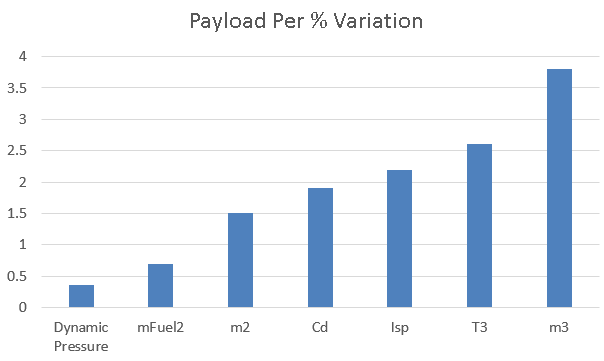
\includegraphics[width=0.99\linewidth]{figures/5_Ascent/BarChartRelativePayloadChange}
\caption{}
\label{fig:BarChartRelativePayloadChange}
\end{figure}



\section{Summary}


In this chapter, LODESTAR was used to design the trajectory of the rocket-scramjet-rocket multi-stage launch system incorporating the SPARTAN scramjet-powered accelerator. 
A trajectory was simulated in which the SPARTAN stage flies at a constant dynamic pressure, producing \PayloadToOrbitConstq kg of payload-to-orbit. 
A trajectory optimised for maximum payload-to-orbit was then calculated, which increased payload mass to heliosynchronous orbit to \PayloadToOrbitStandard kg (an increase of 16.3\%) compared to the constant dynamic pressure trajectory.
  The optimal flight path indicates that the optimal scramjet flight path for a system transitioning between separate airbreathing and rocket-powered stages involves the SPARTAN flying at less than its maximum dynamic pressure at three separate points along the trajectory. 
  Initially, the first stage-SPARTAN separation occurs at a higher trajectory angle than in the constant dynamic pressure trajectory, causing the SPARTAN to fly at lower dynamic pressure. 
  The optimal flight path then exhibits an altitude raising manoeuvre in the middle of the trajectory, which improves the exergy efficiency of the SPARTAN by a very minor 0.003\%$\eta$. 
  Finally, the SPARTAN executes a pull-up manoeuvre before the SPARTAN-third stage separation. This optimal pull-up manoeuvre trades off velocity (a decrease of 116.2m/s) for altitude (an increase of 9.48km) and improved flight path angle (an increase of 10.45$^\circ$), when compared to the constant dynamic pressure case. 
  These conditions improve the exergy efficiency of the third stage rocket significantly, by 3.456\%$\eta$, an increase of 20.5\% over the third stage released from a constant dynamic pressure trajectory. 
 The pull up manoeuvre in the payload-to-orbit optimised trajectory also reduces the maximum dynamic pressure experienced by the third stage to 10.8kPa, a decrease of 43.4kPa compared to a trajectory with minimum pull-up, which allows future benefits due to heat shield mass reduction.  

A sensitivity study was conducted, to determine the relative effects of key vehicle design parameters on the optimised trajectory. 
It was observed that the efficiency trade-off between the first stage and the SPARTAN depends primarily on the pitching ability of the first stage, so that when the first stage is capable of pitching more rapidly, the trade-off shifts in favour of the SPARTAN. 
It was also observed that when the overall magnitude of 'useful' energy utilised during the SPARTAN acceleration is increased, the trade-off between the efficiency of the SPARTAN and the third stage rocket shifts in favour of the SPARTAN, decreasing the size of the pull-up before SPARTAN-third stage separation. 
It was found that the maximum dynamic pressure has a relatively small effect on the payload-to-orbit performance of the launch system, varying the payload-to-orbit by only +24.2kg (+12.8\%) at 60kPa and -20.5kg (-10.8\%) at 40kPa. The negative effect on the payload-to-orbit when flying at 40kPa is likely to be offset by the lower TPS and structural mass required by lower dynamic pressure flight. If the TPS and structural mass decrease is greater than -26.5kg for every 1kPa reduction in the maximum dynamic pressure, then flying at lower dynamic pressure is potentially preferable. 
The specific impulse of the third stage rocket was found to produce the most overall effect on the payload-to-orbit, increasing the payload by +45.9kg (+24.26\%) at 105\% $I_{sp}$, and decreasing the payload by -45.9kg (-24.26\%) at 95\% $I_{sp}$. However, increasing the specific impulse of the third stage rocket is likely to come at a high cost premium, which may be undesirable as the third stage is non-reusable. 
The third stage aerodynamic performance was found to have negligible effect on the payload-to-orbit, indicating this is not a significant design factor. 
The specific impulse of the SPARTAN, the aerodynamic performance of the SPARTAN, the SPARTAN structural mass, and the SPARTAN fuel mass were also varied, and the magnitudes of their payload-to-orbit sensitivities compared. 
These sensitivity comparisons may be useful in driving future design decisions. 





